\documentclass[preprints,review,accept,moreauthors,pdftex]{Definitions/mdpi}

\usepackage{mathrsfs} 
\usepackage[mathscr]{euscript}
\usepackage{amssymb,amsbsy,amsmath,amsfonts}
\usepackage{slashed}
\usepackage{nicefrac}

\def\beq{\begin{equation}}
\def\eeq{\end{equation}}
\def\bea{\begin{eqnarray}}
\def\eea{\end{eqnarray}}

\def\eqlab#1{\label{eq:#1}}
\def\figlab#1{\label{fig:#1}}
\def\tablab#1{\label{tab:#1}}
\def\seclab#1{\label{sec:#1}}

\def\eref#1{(\ref{eq:#1})}
\def\Eqref#1{Eq.~(\ref{eq:#1})}
\def\fref#1{\ref{fig:#1}}
\def\Figref#1{Figure~\ref{fig:#1}}
\def\Tabref#1{Table \ref{tab:#1}}
\def\secref#1{Section \ref{sec:#1}}

\def\boxfrac#1#2{\mbox{$\frac{#1}{#2}$}}
\def\al{\alpha}
\def\be{\beta}
\def\ga{\gamma} \def\Ga{{\it\Gamma}}
\def\de{\delta} \def\De{\Delta}
\def\veps{\varepsilon}  \def\eps{\epsilon}
\def\kp{\kappa}
\def\la{\lambda} \def\La{{\Lambda}}
\def\si{\sigma} \def\Si{{\Sigma}}
\def\th{\theta} \def\vth{\vartheta} \def\Th{\Theta}
\def\w{\omega} \def\W{\Omega} \def\hw{\hat{\omega}}
\def\vfi{\varphi}\def\vphi{\varphi}

\def\scA{\mathscr{A}}
\def\scO{\mathscr{O}}


\def\pa{\partial}
\def\vrho{\varrho}
\def\barf{\zeta}
\def\ie{{i.e., }}
\def\eg{{e.g.\ }}
\def\pa{\partial}
\def\nn{\nonumber}
\def\dd{\mathrm{d}}

\def\bn{\boldsymbol{n}}

\DeclareMathOperator\arctanh{arctanh}
\DeclareMathOperator\im{Im}
\def\ol#1{\overline{#1}}
\def\half{\mbox{\small{$\frac{1}{2}\;$}}}

\firstpage{1} 
\makeatletter 
\setcounter{page}{\@firstpage} 
\makeatother
\pubvolume{xx}
\issuenum{1}
\articlenumber{5}
\pubyear{2019}
\copyrightyear{2019}
\history{}

\pdfoutput=1


\Title{Nucleon Polarizabilities and Compton Scattering as a Playground for Chiral Perturbation Theory}

\newcommand{\orcidauthorA}{0000-0002-2017-7132} 

\Author{Franziska Hagelstein $^{1}$\orcidA{}}

\AuthorNames{Franziska Hagelstein}

\address{%
$^{1}$ \quad Albert Einstein Center for Fundamental Physics, Institute for Theoretical Physics, University of Bern, Sidlerstrasse 5, CH-3012 Bern, Switzerland; hagelstein@itp.unibe.ch}

\abstract{I give a summary of recent results on nucleon polarizabilities, with emphasis on chiral perturbation theory. The predictive calculations of Compton scattering off the nucleon are compared to recent empirical determinations and lattice QCD calculations of the  polarizabilities, thereby testing chiral perturbation theory in the single-baryon sector. }

\keyword{Chiral Perturbation Theory, Proton, Neutron, Compton Scattering, Structure Functions, Polarizabilities, Dispersion Relations}

\begin{document}

\section{Introduction}



The name Chiral Perturbation Theory ($\chi$PT) was first introduced in the seminal works of \citet{Pagels:1974se}, who used
it to describe a systematic expansion in the pion mass
$m_\pi$, which is small compared to other hadronic scales.
Some years later, in 1979, Weinberg \cite{Weinberg:1978kz} made an enlightening  proposal for effective-field theories (EFT) and
the $\chi$PT acquired its present meaning by Gasser and Leutwyler  \cite{Gasser:1983yg,Gasser:1987rb} in this, more powerful, connotation. Since then, $\chi$PT stands for a low-energy EFT of the strong sector of the Standard Model. Written in terms of hadronic degrees of freedom, rather than quarks and gluons, it offers
an efficient way of calculating low-energy hadronic physics. 
Many calculations can be done analytically in a systematic perturbative expansion, in contrast 
to the \textit{ab initio} calculations, viz., lattice QCD, Dyson-Schwinger equations, and other non-perturbative
calculations in terms of quark and gluon fields.  

\begin{figure}[t]
\centering
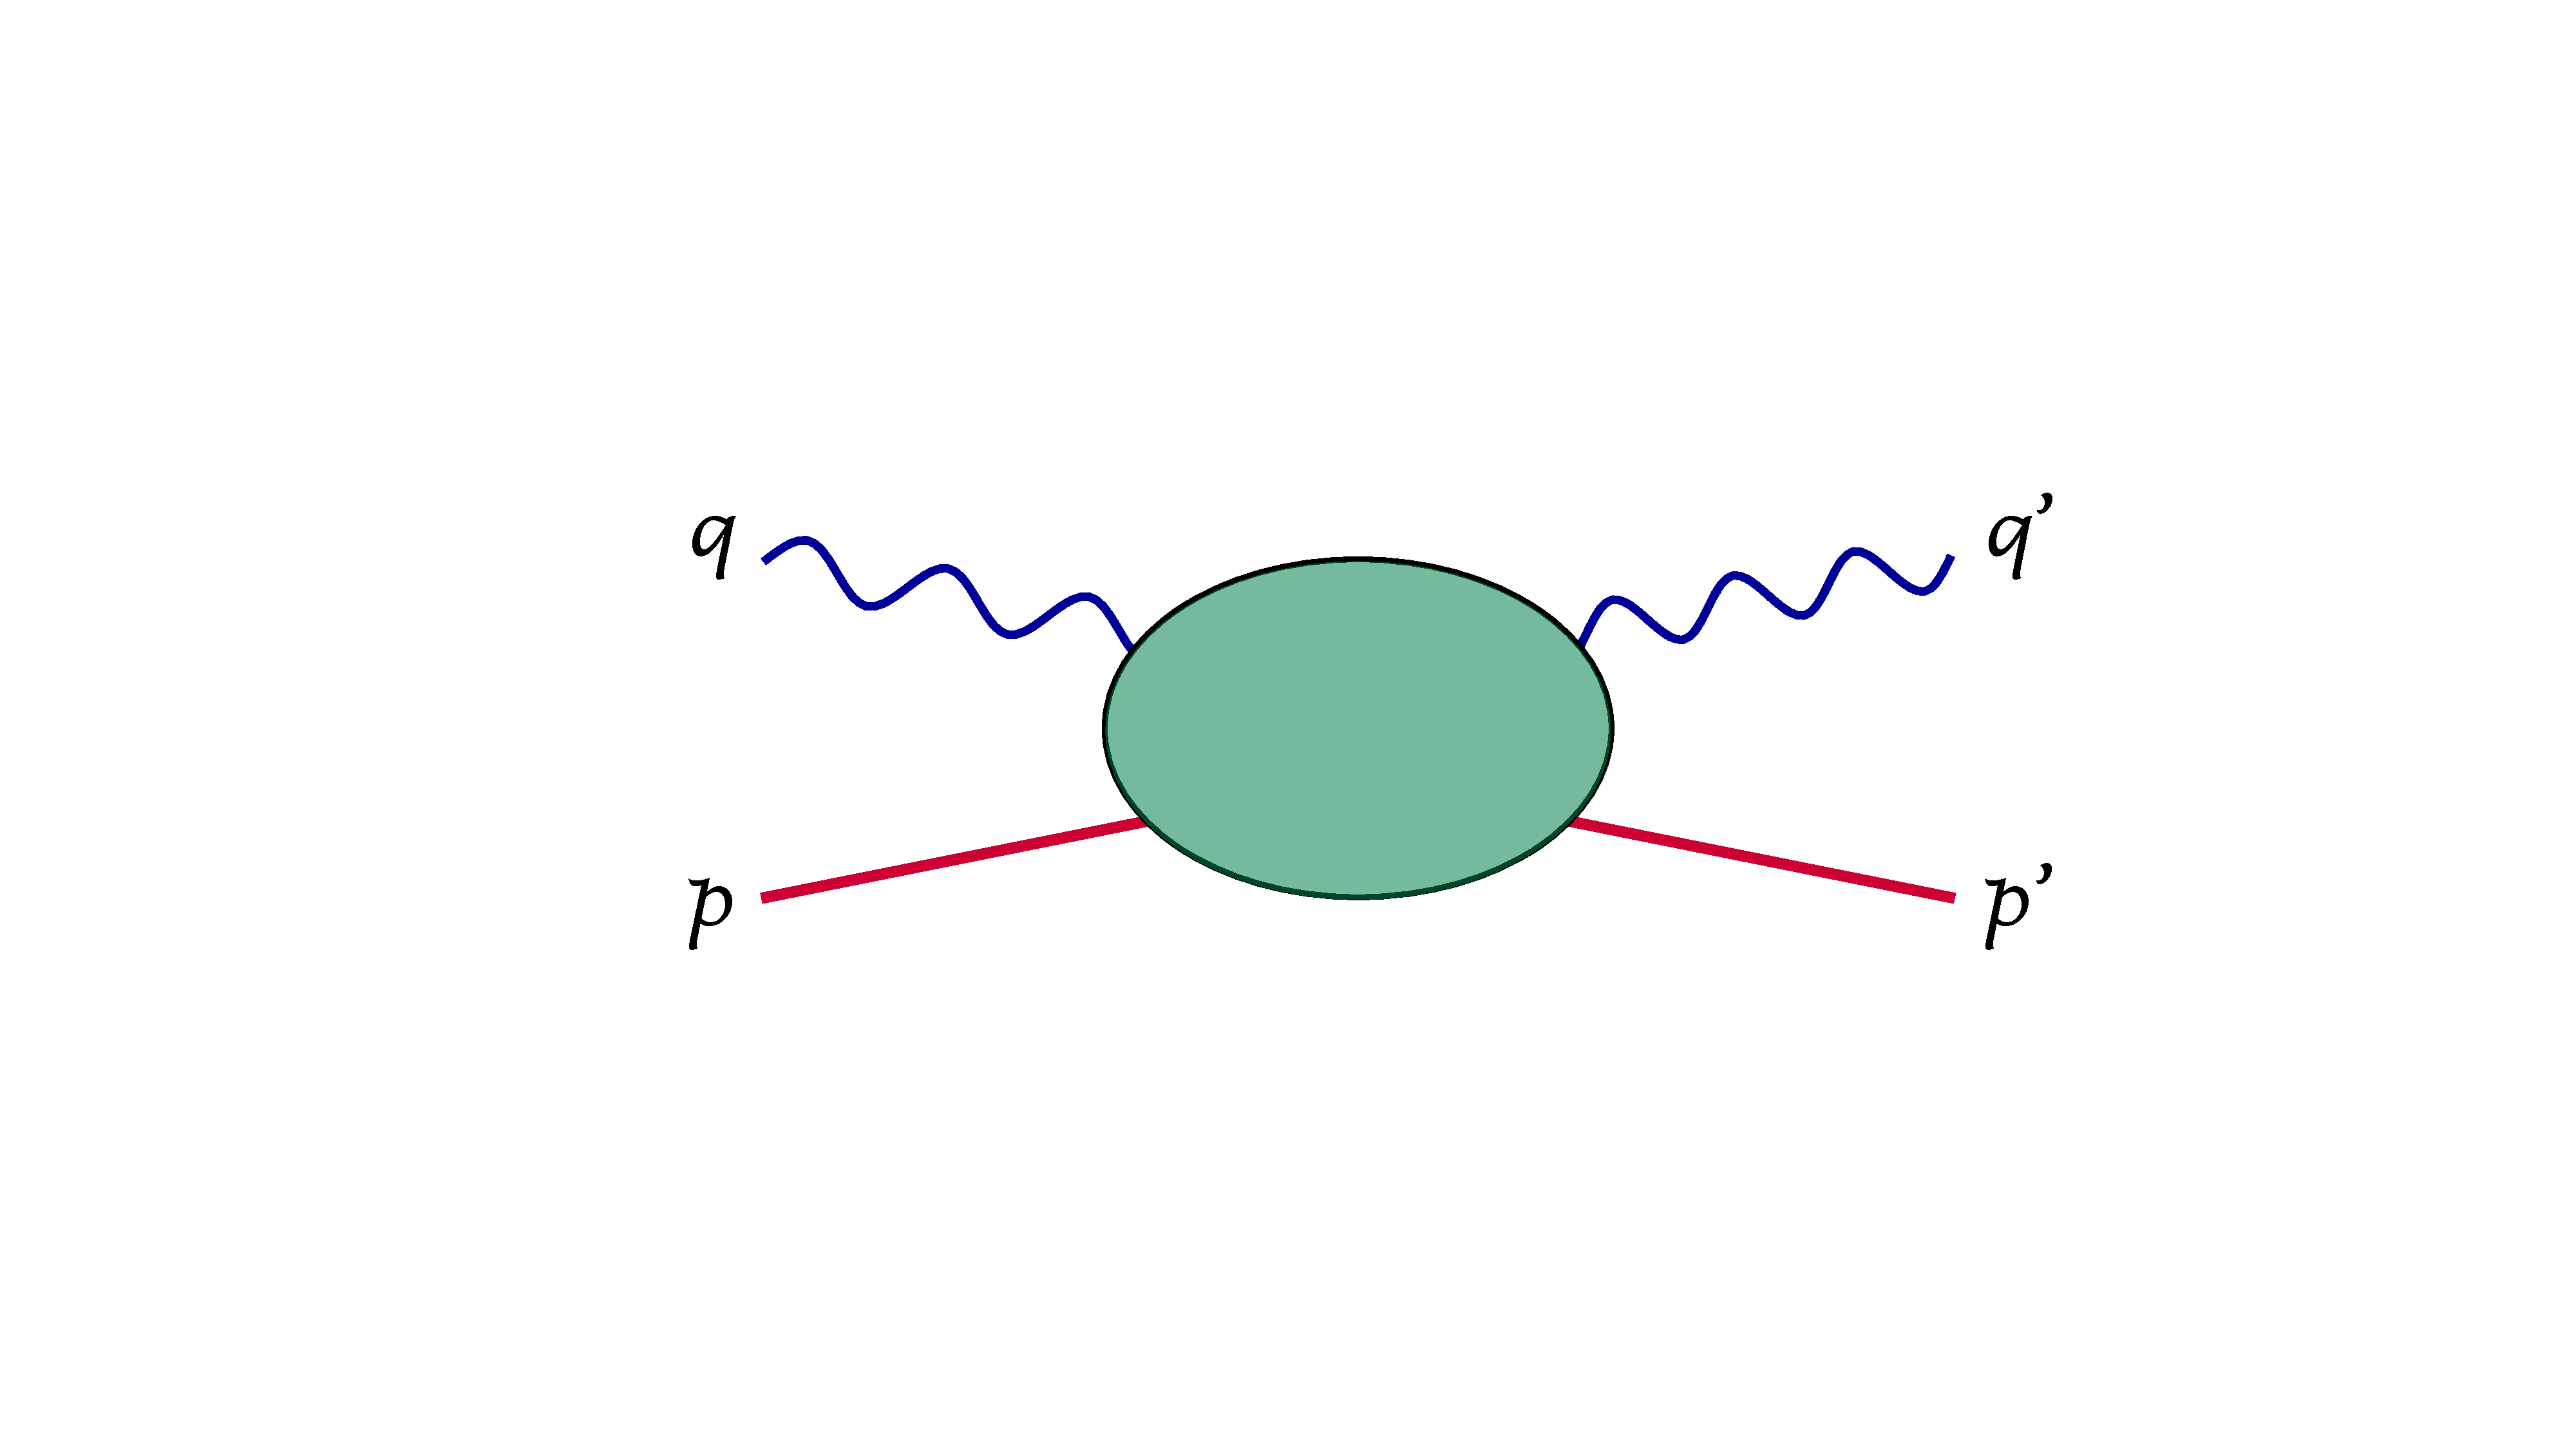
\includegraphics[width=5 cm]{Figures/newCSfigure.pdf}
\caption{Compton scattering off the nucleon in general kinematics: $\gamma^*(q) N(p) \rightarrow \gamma^*(q') N(p')$. \label{CSfigure}}
\end{figure} 

However, as in any EFT framework, the convergence and the predictive power of $\chi$PT calculations are often of concern.
After all, the expansion in energy and momenta is not
as clear-cut as usual expansions in a small coupling constant. And, each new order brings more and more free parameters --- the low-energy constants (LECs). This is why the
cases where $\chi$PT provides true predictions are very valuable. One such case, considered here, is the process of Compton scattering (CS) off the nucleon, see Figure \ref{CSfigure}. It allows one to study the low-energy properties of the nucleon \cite{Bernard:1991rq,Bernard:1991ru}.

The nucleon is characterized by a number
of different polarizabilities, the most important of which 
are the electric and magnetic dipole polarizabilities $\alpha_{E1}$ and $\beta_{M1}$. These quantities describe the size of the electric and magnetic dipole moments induced by an external electric $\vec{E}$ or magnetic $\vec{H}$ field: 
\begin{subequations}
\begin{eqnarray}
\vec{d}_\mathrm{ind.} &=& 4\pi \alpha_{E1} \vec{E},\\
\vec{\mu}_\mathrm{ind.} &=& 4\pi \beta_{M1} \vec{H}.
\end{eqnarray}
\end{subequations}
In loosely bound systems, such as atoms and molecules, these
polarizabilities are roughly given by the volume of the system.
In the nucleon, the sum of dipole polarizabilities is of the order of $10^{-3}$ fm$^3$. This is much smaller than the volume of the nucleon ($\sim 1$ fm$^3$), telling us that it is a much more rigid object. 
There are other important polarizabilities, related to the spin of the nucleon, and therefore called the spin polarizabilities. These are more difficult to visualise in a classical picture.  
Nonetheless, $\chi$PT provides robust predictions for these quantities at leading and next-to-leading order. Given
the accurate empirical knowledge 
of the nucleon polarizabilities from dispersive sum rules and CS experiments,  they become an important benchmark for $\chi$PT in the single-baryon sector. But they are not just a testing ground for $\chi$PT. The lattice QCD studies of nucleon polarizabilities are also closing in on the physical pion mass, see Figures~\ref{alphaE1Pol} and \ref{betaM1Pol}.


This mini-review is by no means comprehensive. A more proper review can be found in  Ref.~\cite{Hagelstein:2015egb}, whereas here I primarily provide an update on the nucleon polarizabilities. For the reader interested in the update only, I recommend to skip to Section \ref{results} where a description of all summary plots is given. A recent theoretical discussion of nucleon polarizabilities in $\chi$PT and beyond can be found in Ref.~\cite{Lensky:2019pye}. Other commendable reviews include: \citet{Guichon:1998xv} or \citet{Fonvieille:2019eyf} (VCS and generalized polarizabilities), \citet{Drechsel:2002ar} or \citet{Pasquini:2018wbl} (dispersion relations for CS), \citet{Pascalutsa:2006up} ($\Delta(1232)$ resonance), \citet{Phillips:2009af} (neutron polarizabilities), \citet{Griesshammer:2012we} ($\chi$EFT and RCS experiments), \citet{Holstein:2013kia} (pion, kaon, nucleon polarizabilities), \citet{Geng:2013xn} (B$\chi$PT), \citet{Pascalutsa:2018ced} (dispersion relations), \citet{Deur:2018roz} (nucleon spin structure). A textbook introduction to $\chi$PT can be found in Ref.~\cite{Scherer2012}.



The paper is organized as follows. In Sections \ref{BChPTintro} and \ref{CSintro}, I briefly describe the $\chi$PT framework and the CS formalism. In Section \ref{results}, I summarize recent $\chi$PT results for the nucleon polarizabilities and compare to empirical and lattice QCD evaluations. 



\section{Baryon Chiral Perturbation Theory} \label{BChPTintro}



The low-energy processes involving a nucleon, such as $\pi N$ scattering or CS off the nucleon, can be described by SU(2) baryon chiral perturbation theory (B$\chi$PT), which is the manifestly Lorentz-invariant variant of $\chi$PT in the single-baryon sector \cite{Gasser:1987rb,Gegelia:1999gf,Fuchs:2003qc}. To introduce it, I will start in Section \ref{NuclPC} with the basic EFT including only pions and nucleons. Then, in Section \ref{DeltaPC}, I will discuss different ways (counting schemes) for incorporation of the lowest nucleon excitation --- the $\Delta(1232)$ resonance --- into the $\chi$PT framework. In Section \ref{LECsec}, I will show how the LECs can be fit to experimental data and discuss the predictive power of $\chi$PT for CS. In Section \ref{secHB}, I introduce the heavy-baryon chiral perturbation theory (HB$\chi$PT) and point out how its predictions differ from B$\chi$PT for certain polarizabilities. For more details on B$\chi$PT for CS, I refer to the following series of calculations: RCS \cite{Lensky:2008re,Lensky:2009uv,Lensky:2015awa}, VCS \cite{Lensky:2016nui} and forward VVCS \cite{Lensky:2014dda,Alarcon:2020wjg, Alarcon:2020icz}.

\begin{figure}[t]
\centering
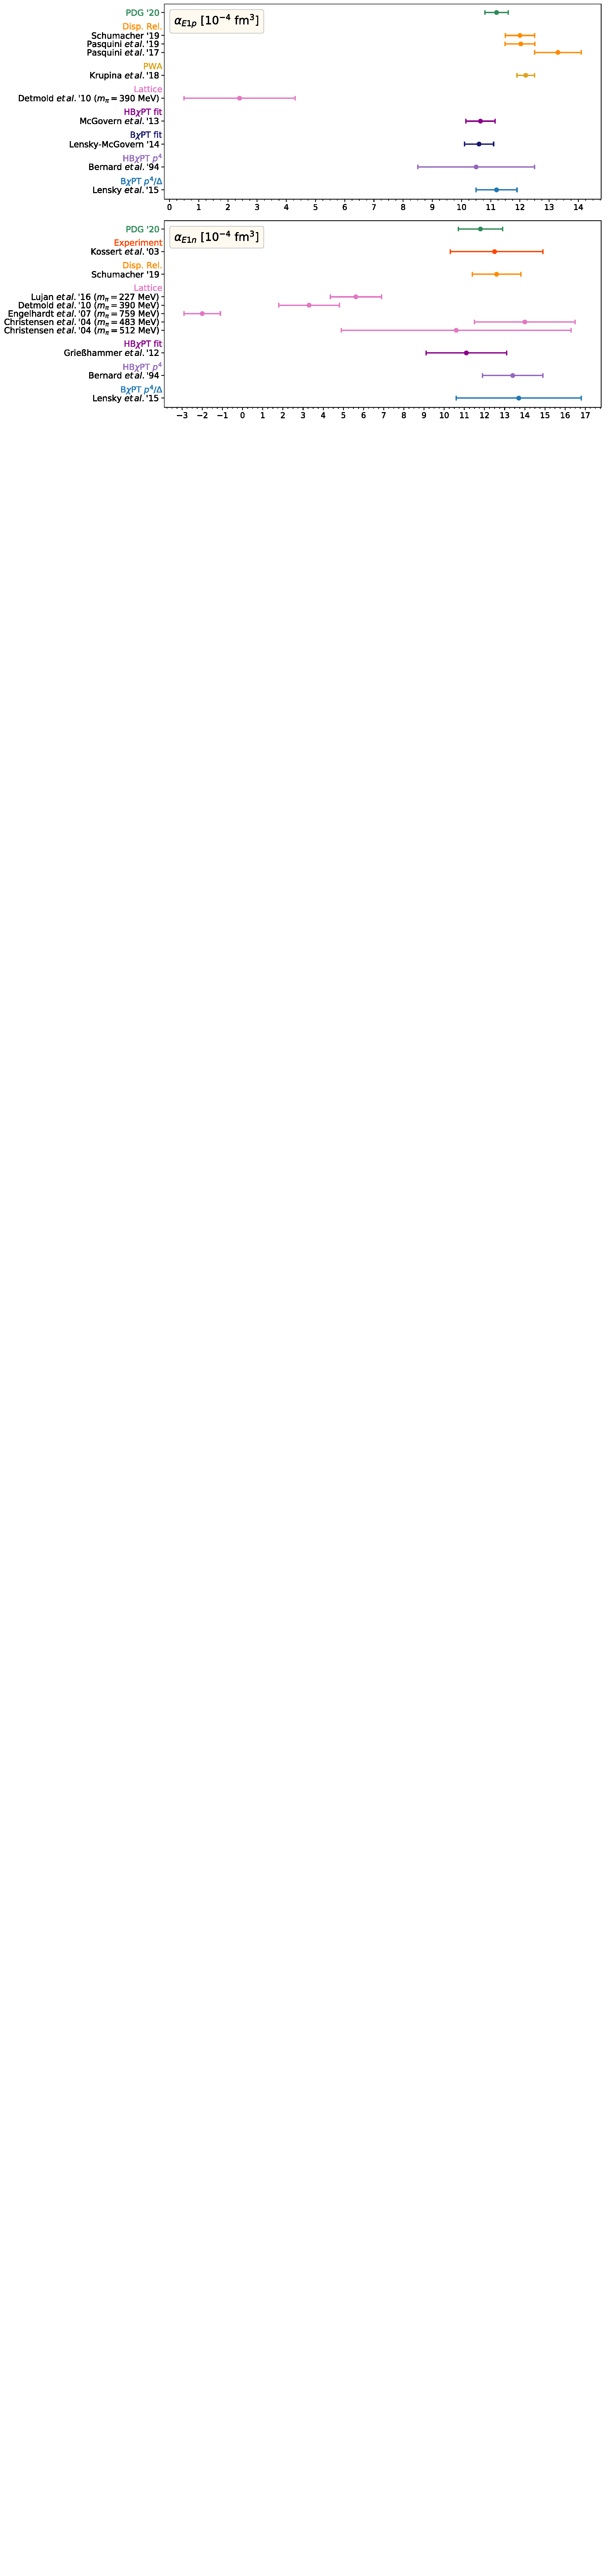
\includegraphics[width=\columnwidth]{Figures/alphaE1Pol.pdf}
\caption{Electric dipole polarizability $\al_{E1}$ of the nucleon. \label{alphaE1Pol}}
\end{figure} 



\subsection{B$\chi$PT with pions and nucleons}
\label{NuclPC}
 Consider the basic version of SU(2) B$\chi$PT including only pion and nucleon fields \cite{Gasser:1987rb}: scalar iso-vector $\pi^a(x)$ and spinor iso-doublet $\mathcal{N}(x)$. Expanding the EFT Lagrangian \cite{Gasser:1987rb}  to leading orders in pion derivatives,  mass and fields, one finds (see, e.g., Ref.~\cite{Ledwig:2011cx}):
\begin{subequations}
\eqlab{PionLagrangians}
\bea
\mathcal{L}^{(1)}_\mathcal{N}&=&\ol{\mathcal{N}} \big(\slashed{D}-M_N\big)\mathcal{N}-\frac{g_A}{2f_\pi}\ol{\mathcal{N}}\, \tau^a \left(\slashed{D}^{ab} \pi^b\right)\gamma_5\, \mathcal{N},\eqlab{piNN}\\
\mathcal{L}^{(2)}_\pi&=&\frac{1}{2} \Big(D_\mu^{ab} \pi^b\Big)\Big(D^\mu_{ac} \pi^c\Big)-\frac{1}{2}m_\pi^2 \pi_a\pi^a,\eqlab{pionLag}
\eea
\end{subequations}
with the covariant derivatives:
\begin{subequations}
\bea
D_\mu^{ab} \pi^b&=&\delta^{ab} \partial_\mu \pi^b+ieQ_\pi^{ab}A_\mu\pi^b,\\
D_\mu \mathcal{N}&=&\partial_\mu \mathcal{N}+ieQ_N A_\mu\mathcal{N}+\frac{i}{4f_\pi^2}\,\varepsilon^{abc}\tau^a \pi^b (\partial_\mu \pi^c),
\eea
\end{subequations}
the photon vector field $A_\mu(x)$,
and the charges:
\begin{subequations}
\bea
Q_\pi^{ab}&=&-i \varepsilon^{ab3},\\
Q_N&=&\half \!(1+\tau^3).
\eea
\end{subequations}
Here, $\tau^a$ are the Pauli matrices, $\ga_5 = i \ga^0\ga^1\ga^2\ga^3$ are the Dirac matrices, and all other parameters are introduced in Table \ref{LECtable}. 

The key ingredient for the development of $\chi$PT as a low-energy EFT of QCD was the 
observation that the pion couplings are proportional to their four-momenta \cite{Weinberg:1978kz,Gasser:1983yg,Gasser:1987rb}. Therefore, at
low momenta the couplings are weak and a perturbative expansion is possible. This chiral expansion is done in powers of pion momentum and mass, commonly denoted as $p$, over the scale of spontaneous chiral symmetry breaking, $\Lambda_{\chi\mathrm{SB}}\sim 4 \pi f_\pi \approx 1$ GeV.  Therefore, one expects that $\chi$PT provides a systematic description of the strong interaction at energies well below $1$ GeV. Considering only pion and nucleon fields, the chiral order $\mathcal{O}(p^{n})$ of a Feynman diagram with $L$ loops, $N_\pi$ ($N_N$) pion (nucleon) propagators, and $V_k$ vertices from $k$-th order Lagrangians [e.g., $k=1$: $\Gamma^\mu_{\gamma NN}$ interaction from \Eqref{piNN}, $k=2$: $\Gamma^\mu_{\gamma\pi\pi}$ interaction from \Eqref{pionLag}] is defined as \cite{Gasser:1987rb}:
\beq
n=4L-2N_\pi-N_N+\sum_k k\, V_k.
\eeq







In the case of CS, the low-energy scale $p$ also includes the photon energy $\nu$ and virtuality $Q$, which therefore should be much smaller than $1$ GeV. 
However, the presence of bound states or low-lying resonances may lead to a breakdown of this perturbative expansion.   For example, in $\pi \pi$ scattering the limiting scale of the perturbative expansion is set by the $\sigma(600)$ and $\rho(775)$ mesons  \cite{Colangelo:2001df,Caprini:2005an}. In the single-nucleon sector, the breakdown
scale is set by the excitation energy of the first nucleon resonance, the $\Delta(1232)$ isobar.  
That is unless the $\Delta(1232)$ is included explicitly in the effective Lagrangian.



\subsection{Inclusion of the $\Delta(1232)$ and Power Counting}\label{DeltaPC}

The $\Delta(1232)$ resonance as the lightest nucleon excitation has an excitation energy
\beq
\varDelta = M_\Delta - M_N \simeq 293\, \mathrm{MeV},
\eeq
which is in the same ballpark as the pion mass. In the following, it will be included as an explicit degree of freedom: vector-spinor iso-quartet $\Delta_\mu(x)$. The relevant Lagrangians read~\cite{Ledwig:2011cx,Pascalutsa:2005ts,Pascalutsa:2005vq}:
\begin{subequations}
\eqlab{DeltaLagrangians}
\bea
\mathcal{L}^{(1)}_\Delta&=&\ol{\Delta}_\mu \left(i \gamma^{\mu \nu \lambda}D_\lambda -M_\Delta \gamma^{\mu \nu}\right) \Delta_\nu+\frac{H_A}{2f_\pi M_\Delta}\,\varepsilon^{\mu \nu \al \lambda}\,\ol \Delta_\mu \mathscr{T}^{\,a} \left(D_\al \Delta_\nu\right)D_\lambda^{ab}\pi^b,\qquad\quad\\
\mathcal{L}^{(1)}_{\pi\Delta \mathcal{N}}&=&\frac{i h_A}{2f_\pi M_\Delta} \ol{\mathcal{N}} \,T^a\gamma^{\mu \nu \lambda}\left(D_\mu \Delta_\nu\right)\left(D_\lambda^{ab}\pi^b\right)+\text{h.c.},\\
\eqlab{nmGammaNDeltaLag}
 \mathcal{L}^{(2) \,\mathrm{non-minimal}}_{\gamma N \Delta}&=&\frac{3e}{2M_N(M_N+M_\Delta)}\Bigg[\bar{N} T_3\Big\{i g_M (\partial_\mu \Delta_\nu) \tilde{F}^{\mu \nu}-g_E  \gamma_5 (\partial_\mu \Delta_\nu) F^{\mu \nu}\eqlab{LagrangianGND}\\
 &&+i \frac{g_\mathrm{C}}{M_\Delta}\gamma_5 \gamma^\al (\partial_\al \Delta_\nu-\partial_\nu \Delta_\al)\partial_\mu F^{\mu \nu}\Big\}+\text{h.c.}\Bigg],\nn
\eea
\end{subequations}
with the
covariant derivative:
\beq
D_\mu \Delta_\nu= \partial_\mu \Delta_\nu+ie Q_\Delta A_\mu \Delta_\nu+\frac{i}{2f_\pi^2} \,\varepsilon^{abc}\, \mathscr{T}^a\pi^b(\partial_\mu \pi^c),
\eeq
and the
charge:
\beq
Q_\Delta=\half \!(1+3 \mathscr{T}^3).
\eeq
Here, h.c.\ stands for the hermitian conjugate, $\gamma^{\mu \nu}=-\frac{i}{2}\epsilon^{\mu \nu \al \be}\ga_\al \ga_\be \ga^5$ and $\gamma^{\mu \nu \al}=-i\epsilon^{\mu \nu \al \be} \ga_\be \ga^5$ are Dirac matrices with $\epsilon_{0123}=1$, and $T^a$ ($\mathscr{T}^a$) are the isospin $1/2$ ($3/2$) to $3/2$ transition matrices. The latter commute with the Dirac matrices. The superscripts of the Lagrangians in Eqs.~\eref{PionLagrangians} and \eref{DeltaLagrangians} denote their order as reflected by the number of comprised small quantities: pion mass, momentum and factors of $e$. Inclusion of the $\Delta(1232)$ introduces the excitation energy $\varDelta$ as another small scale, which has to be considered when defining a power-counting for the perturbative $\chi$PT expansion. 

\begin{figure}[t]
\centering
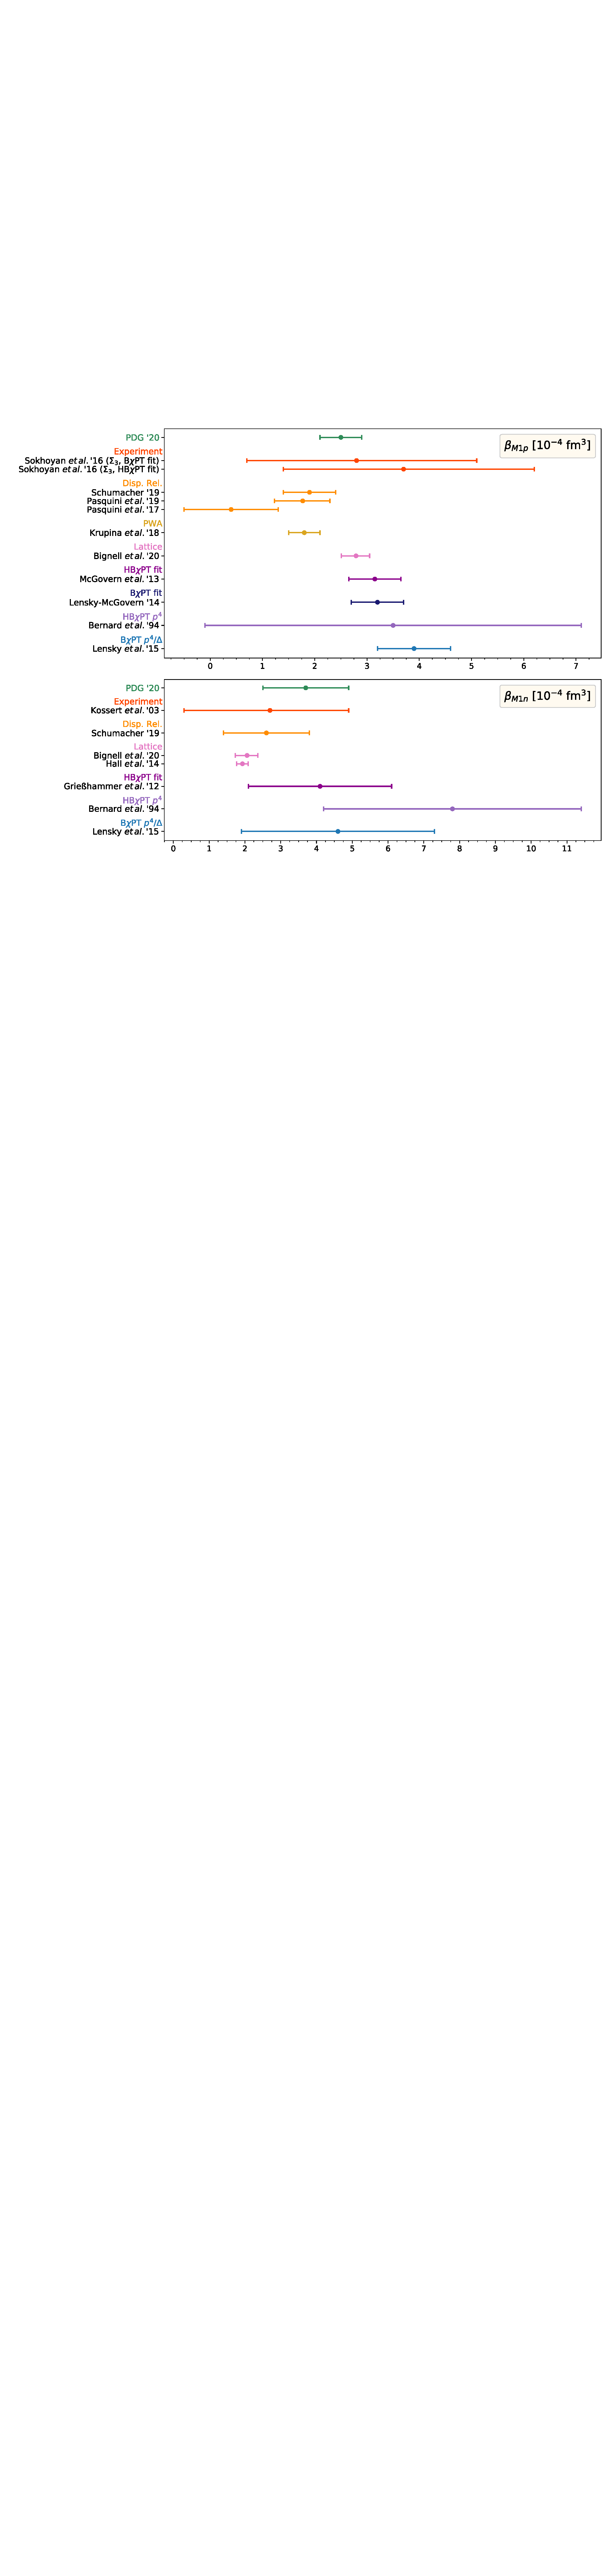
\includegraphics[width=\columnwidth]{Figures/betaM1Pol.pdf}
\caption{Magnetic dipole polarizability $\be_{M1}$  of the nucleon. \label{betaM1Pol}}
\end{figure} 




There are two prominent counting schemes for $\chi$PT with explicit inclusion of the $\Delta(1232)$.
For simplicity, they both deduce a single expansion parameter from the two involved small mass scales: $\epsilon=m_\pi/\Lambda_{\chi\mathrm{SB}}$ and 
$\delta=\varDelta/\Lambda_{\chi\mathrm{SB}}$. In the $\eps$-expansion (small-scale expansion) it is assumed that $\eps \sim \delta$ \cite{Hemmert:1996xg}, while in the $\delta$-expansion one assumes $\eps \sim \delta^2$ with $\eps \ll \delta$ \cite{Pascalutsa:2003aa}. In this way, the $\delta$-expansion defines a hierarchy between the two mass scales. Consequently, it defines two regimes where the $\Delta(1232)$ contributions need to be counted differently:
\begin{itemize}[leftmargin=*,labelsep=5.8mm]
\item low-energy region: $p \sim m_\pi$;
\item resonance region: $p\sim \varDelta$.
\end{itemize}
This makes sense since the $\Delta(1232)$ is expected to be suppressed at low energies and dominating in the resonance region. The chiral order $\mathcal{O}(p^{n_\delta})$ of a Feynman diagram with $N_\text{1$\Delta$R}$ ($N_\text{1$\Delta$I}$)  one-$\Delta$-reducible (one-$\Delta$-irreducible) propagators is in the $\delta$-expansion defined as:
\beq
n_\delta=\begin{cases}n-\nicefrac{1}{2}N_\Delta&p\sim m_\pi,\\
n-3N_\text{1$\Delta$R}-N_\text{1$\Delta$I}&p\sim\Delta,\eqlab{deltacounting}
\end{cases}
\eeq
where
\beq
N_\Delta=N_\text{1$\Delta$R}+N_\text{1$\Delta$I}.
\eeq
An extensive review on the electromagnetic excitation of the $\Delta$(1232)-resonance with more details on the formulation of the extended $\chi$PT framework and the chiral expansion in the resonance region can be found in Ref.~\cite{Pascalutsa:2006up}. 
As we will see in Section \ref{results}, B$\chi$PT calculations based on the
$\eps$ \cite{Bernard:2012hb} and the
$\de$ \cite{Lensky:2014dda,Alarcon:2020icz} counting scheme give significantly different predictions for the longitudinal-transverse polarizability of the proton shown in Figure~\ref{LTPolarizabilities}.



\subsection{Low-Energy Constants and Predictive Orders} \label{LECsec}

At any given order in the chiral expansion, the divergencies of the EFT
are absorbed by renormalization of a finite number of LECs.
To match $\chi$PT to QCD as the fundamental theory of the strong interaction, the renormalized LECs need to be fitted to experimental or lattice data. It is important that the LECs are constrained to be of {\it natural size}. Take for instance the
fifth-order forward spin polarizability (in units of $10^{-4}$~fm$^6$) \cite{Alarcon:2020icz}:
\begin{subequations}
\begin{align}
&\bar\gamma_{0p} =1.12(30)\approx 2.08\,\mbox{($\pi$N loop)} -0.96\,\mbox{($\Delta$ exchange)} -0.01\, \mbox{($\pi\Delta$ loop)}, \label{Eq:gamma0ProtonRealPoint}\\
&\bar\gamma_{0n} =1.95 (30) \approx 2.92\,\mbox{($\pi$N loop)}-0.96\,\mbox{($\Delta$ exchange)} -0.01\, \mbox{($\pi\Delta$ loop)}.
\end{align}
\end{subequations}
The next-to-leading-order effect of the $\Delta(1232)$ is two to three times smaller than the leading-order effect of the pion cloud. This is consistent with estimates from power counting, according to which each subleading order is expected to be suppressed with respect to the previous one by a factor of $\sim\varDelta/M_N\sim 1/3$.
Therefore, implementing this {\it naturalness} allows to estimate the uncertainty due to neglect of higher-order effects.

The LECs entering a next-to-next-to-leading-order B$\chi$PT calculation of low-energy CS in the $\delta$-expansion are $f_\pi$, $g_A$, $h_A$, $g_M$, $g_E$ and $g_C$.\footnote{Note that the $g_E$ and $g_C$ couplings of the $N$-to-$\Delta$ transition would be strictly speaking of higher order.} They are listed in Table \ref{LECtable} together with the experiments used to constrain their values. As one can see, B$\chi$PT has 
``predictive power'' for CS up to and including $\mathcal{O}(p^4/\varDelta)$ because all relevant LECs are matched to processes other than CS.\footnote{Note that $\mathcal{O}(p^4/\varDelta)$ corresponds to $\mathcal{O}(p^{7/2})$, cf.\ \Eqref{deltacounting} with $p
^{1/2} \sim \varDelta $ or $p \sim m_\pi$.} This makes $\chi$PT the perfect tool to study the low-energy structure of the nucleon as encoded in CS and the associated polarizabilities. Starting from $\mathcal{O}(p^4)$, LECs need to be fitted to the CS process as well, for instance through the Baldin sum rule, as done in  Refs.~\cite{McGovern:2012ew,Griesshammer:2012we,Lensky:2014efa,Griesshammer:2015ahu,Alarcon:2020wjg}. 

\begin{figure}[t]
\centering

\includegraphics[width=\columnwidth]{Figures/QuadrupolePol.pdf}
\caption{Quadrupole polarizabilities $\al_{E2}$ and $\be_{M2}$ of the proton. \label{QuadrupolePol}}
\end{figure} 





\subsection{Heavy-Baryon Expansion}\label{secHB}

The theory of HB$\chi$PT  was first introduced in Ref.~\cite{Jenkins:1990jv}, and later applied to CS and polarizabilities \cite{Butler:1992ci}, including also the effect of the $\Delta(1232)$ \cite{Bernard:1995dp,Hemmert:1996rw,Hildebrandt:2003fm,Griesshammer:2012we,Kao:2002cp,Kao:2003jd,Nevado:2007dd}. The results of HB$\chi$PT can be recovered from the B$\chi$PT results by expanding in powers of the inverse nucleon mass. HB$\chi$PT calculations tend to fail in describing the $Q
^2$ evolution of the generalized nucleon polarizabilities \cite{Alarcon:2020icz,Alarcon:2020wjg}. 
Also for the static polarizabilities the heavy-baryon expansion can give significantly different predictions. Consider for instance the nucleon dipole polarizabilities. The B$\chi$PT prediction (in units of $10^{-4}\,$fm$^3$) \cite{Lensky:2015awa}:
\begin{subequations}
\begin{eqnarray}
\eqlab{alChPT}
 \alpha_{E1p}&=& 6.9\,\mbox{($\pi$N loop)} -0.1\,\mbox{($\Delta$ exchange)} + 4.4\, \mbox{($\pi\Delta$ loop)} = 11.2\pm 0.7,\\
\beta_{M1p}&=&-1.8\,\mbox{($\pi$N loop)} + 7.1\,\mbox{($\Delta$ exchange)}-1.4\, \mbox{($\pi\Delta$ loop)} =3.9\pm 0.7,
\end{eqnarray}
\end{subequations}
is in good agreement with empirical evaluations, see Figs.~\ref{alphaE1Pol} and \ref{betaM1Pol}.
%\begin{subequations}
%\eqlab{abHBChPT}
%\bea 
%  \alpha_{E1}^{(p)}(\mbox{HB}) &=& 12.2 \,\mbox{($\pi$N loop)} + 0 \,\mbox{($\Delta$ exchange)} + 8.6 \, \mbox{($\pi\Delta$ loop)}  = 20.8\,,\\
% \beta_{M1}^{(p)}(\mbox{HB})&=& 1.2 \,\mbox{($\pi$N loop)}  
% + 12 \,\mbox{($\Delta$ exchange)} +1.5 \,  \mbox{($\pi\Delta$ loop)} = 14.7  \,.
%\eea 
%\end{subequations}
In HB$\chi$PT, however, the $\De(1232)$ contributions
to the nucleon polarizabilities turn out to be large \cite{Hemmert:1996rw}
and need to be canceled by promoting the higher-order [$\mathcal{O}(p^4)$] counterterms $\delta \alpha$ and $\delta \beta$  \cite{Hildebrandt:2003fm}:
\begin{subequations}
\eqlab{abHBChPT}
\bea 
  \alpha_{E1p}(\mbox{HB}) &=& 11.87 \,\mbox{($\pi$N loop)} + 0 \,\mbox{($\Delta$ exch.)} + 5.09 \, \mbox{($\pi\Delta$ loop)} -(5.92\pm 1.36)\, \mbox{($\delta \alpha$)} \nn\\
  &=& 11.04\pm1.36\,,\\
 \beta_{M1p}(\mbox{HB})&=& 1.25 \,\mbox{($\pi$N loop)}  
 + (11.33\pm 0.70) \,\mbox{($\Delta$ exch.)} +0.86\,  \mbox{($\pi\Delta$ loop)}\\
 &&-(10.68\pm 1.17)\, \mbox{($\delta \beta$)}\qquad\nn \\
  &=&  2.76\mp 1.36,
\eea 
\end{subequations}
at the expense of 
violating the naturalness requirement, see also Ref.~\cite{Griesshammer:2012we}. This can be seen from the dimensionless LECs associated to $\delta \alpha$ and $\delta \beta$ \cite{Hildebrandt:2003fm}, $g_{117}=18.82\pm0.79$ and $g_{118}=-6.05\mp 0.66$, that should be of $\mathcal{O}(1)$ to be consistent with estimates from power counting. This problem is
discussed at length in Refs.~\cite{Lensky:2009uv,Hall:2012iw}.




\begin{table}[t]
\caption{Low-energy constants and other parameters and the orders at which they appear in the chiral expansion when employing the low-energy $\delta$-expansion counting scheme. \label{LECtable}}
\centering
\begin{tabular}{ccccc}
\toprule
\textbf{Order in} &	\multicolumn{2}{c}{}&	& \\
\textbf{chiral expansion} &\multicolumn{2}{c}{\multirow{-2}{*}{\textbf{$\chi$PT parameters}}}	& \multirow{-2}{*}{\textbf{Values}}	&\multirow{-2}{*}{ \textbf{Sources}}\\
\midrule
 &fine-structure constant& $\al$ & $\simeq 1/137.04$ &\\
\multirow{-2}{*}{$\mathcal{O}(p^2)$ }&nucleon mass& $M_N$ & $938.27$ MeV &\\
\hline
&nucleon axial charge&$g_A$&$1.27$&neutron decay $n\rightarrow p\,e^-\, \bar\nu_e$ \cite{Olive:2016xmw}\\
 &pion decay constant&$f_\pi$&$92.21$ MeV&pion decay $\pi^+\rightarrow \mu^+ \nu_\mu$ \cite{Olive:2016xmw}\\
 \multirow{-3}{*}{$\mathcal{O}(p^3)$} &  pion mass&$m_\pi$ & $139.57$ MeV &\\
 \hline
 &&&&$P_{33}$ partial wave in $\pi N$ scattering\\
&\multirow{-2}{*}{$N$-to-$\Delta$ axial coupling}&\multirow{-2}{*}{$h_A$}&\multirow{-2}{*}{$2.85$}&and $\Delta(1232)$ decay width \cite{Pascalutsa:2006up,Pascalutsa:2004je,Pascalutsa:2005nd} \\
 &$\Delta(1232)$ mass& $M_\Delta$ & $1232$ MeV &\\
&magnetic (M1) coupling &$g_M$&$2.97$ &\\
& electric (E2) coupling &$g_E$&$-1.0$&\\
\multirow{-6}{*}{$\mathcal{O}(p^4/\varDelta)$} &Coulomb (C2) coupling &$g_\mathrm{C}$&$-2.6$&\multirow{-3}{*}{\shortstack{pion electroproduction\\ $e^- N \rightarrow e^- N \pi$ \cite{Pascalutsa:2005vq}}}\\
\bottomrule
\end{tabular}
\end{table}

\section{Compton Scattering Formalism} \label{CSintro}

The CS process, shown in Figure~\ref{CSfigure}, gives the most direct access to the nucleon polarizabilities. Of interest are the following kinematic regimes, described by the four-momenta of incoming (outgoing) photons $q(q')$ and nucleons $p(p')$:
\begin{itemize}[leftmargin=*,labelsep=5.8mm]
\item	Real Compton scattering (RCS): $q^2=q^{\prime\,2}=0$;
\item	Virtual Compton scattering (VCS): $q^2=-Q^2<0$ and $q^{\prime\,2}=0$;
\item	Forward doubly-virtual Compton scattering (VVCS): $q=q'$ (thus $p=p'$) and $q^2=-Q^2<0$.
\end{itemize}
In general kinematics ($p^2=p^{\prime\,2}=M_N^2$, $q^2 \neq q^{\prime\,2}$), the CS amplitude can be described by $18$ independent tensor structures. For VCS one needs $12$ independent tensor structures; for RCS one needs $6$ independent tensor structures \cite{Hearn:1962zz,Babusci:1998ww}. In the forward limit, this reduces to $4$ independent tensor structures for virtual photons and $2$ independent tensor structures for real photons. 







Splitting into spin-independent (symmetric) and spin-dependent (antisymmetric) parts, the forward VVCS decomposes into the following four scalar amplitudes:
\begin{subequations}
\beq
T^{\mu \nu} (q,p) = \left[T^{\mu \nu}_S+T^{\mu \nu}_A\right] (q,p) ,
\eeq
with
\bea
T^{\mu \nu}_S(q,p) & = & -g^{\mu\nu}\,
T_1(\nu, Q^2)  +\frac{p^{\mu} p^{\nu} }{M_N^2} \, T_2(\nu, Q^2), \eqlab{VVCS_TS}\\
T^{\mu \nu}_A (q,p) & = &-\frac{1}{M_N}\gamma^{\mu \nu \al} q_\al \,S_1(\nu, Q^2) +
\frac{Q^2}{M_N^2}  \gamma^{\mu\nu} S_2(\nu, Q^2),
\eea
\end{subequations}
with $\nu$ the photon lab-frame energy and terms which vanish upon contraction with the photon polarization vectors omitted. For real photons, the following two scalar amplitudes  survive: 
\beq
f(\nu)=\frac{1}{4\pi}T_1(\nu,0), \qquad g(\nu)=\frac{\nu }{4\pi M_N} S_1(\nu,0).
\eeq
Constraints relating the different kinematic regimes (RCS, VCS and forward VVCS) are discussed in Refs.~\cite{Lensky:2017bwi} and \cite{Pascalutsa:2014zna,Lensky:2017dlc} for the unpolarized and polarized CS, respectively. Here, the focus is on RCS and forward VVCS.

\begin{figure}[t]
\centering

\includegraphics[width=\columnwidth]{Figures/DispersivePol.pdf}
\caption{Dispersive polarizabilities $\al_{E1\nu}$ and $\be_{M1\nu}$ of the proton. \label{DispersivePol}}
\end{figure} 

The off-forward RCS is conveniently described by the covariant decomposition~\cite{Pascalutsa:2003aa}: 
\begin{subequations}
\eqlab{CovarAmp}
 \beq
 \bar u^{\,\prime} (\veps' \cdot T \cdot \veps)  u  = 4\pi \al\,\hat \scA^T (s,t)\, \bar u^{\,\prime} \hat \scO^{\mu \nu}  u \,  \mathcal{E}_{\mu}^{\prime }  \mathcal{E}_{\nu},
 \eeq
 with the overcomplete set of $8$ tensors:
  \bea
&& \hat \scA(s,t) = \big\{\scA_1, \, \cdots, \, \scA_8 \big\} (s,t), \\
&& \hat \scO^{\mu\nu} = \big\{ -g^{\mu \nu}, \; q^{\mu} q^{\prime\,\nu},\; 
-\gamma^{\mu \nu},\; g^{\mu \nu} (q' \cdot \gamma \cdot q),\; q^{\mu} q'_{\alpha} \gamma^{\alpha \nu}-\gamma^{\alpha \mu} q_{\alpha} q'^{\nu},\;q^{\mu} q_{\alpha} \gamma^{\alpha \nu}-\gamma^{\alpha \mu} q'_{\alpha} q'^{\nu},\nn \\  
&& \qquad\qquad 
q^{\mu} q^{\prime\,\nu}(q' \cdot \gamma \cdot q) ,\; 
- i \gamma_5 \epsilon^{\mu \nu \alpha \beta} q'_{\alpha} q_{\beta}\big\}, \\
&& \mathcal{E}_{\mu}  = \veps_{\mu} - \frac{P \cdot \veps}{P \cdot q} \, q_{\mu},
\quad \mathcal{E}_{\mu}'  = \veps_{\mu}' - \frac{P \cdot \veps'}{P \cdot q} \, q_{\mu}',
\quad P_\mu = \half (p + p')_\mu, \quad P\cdot q=P\cdot q',
 \eqlab{epsilon_b}
\eea 
\end{subequations}
and the incoming (outgoing) photon polarization vector $\veps^{(\prime)}$ and Dirac spinor $u^{(\prime)}$. Alternatively, one can choose the non-covariant decomposition with the minimal set of $6$ tensors:
\begin{subequations}
\eqlab{helAmp}
\beq
\bar u^{\,\prime} (\veps' \cdot T \cdot \veps)  u =  8\pi \al M_N  \,  \hat A^T (s, t)\, 
 \chi^{\,\prime} \veps_i' \, \hat O_{ij}\,  \veps_j\,  \chi, 
\eeq 
with the incoming (outgoing) Pauli spinor $\chi^{(\prime)}$ and the scalar complex amplitudes:
\bea
&& \hat A(s,t) = \big\{A_1, \, \cdots, \, A_6 \big\} (s,t), \\
&& \hat O_{ij} = \big\{ \de_{ij}, \, n_i n_j',\, i \eps_{ijk} \si_k,\, \de_{ij}
 i \eps_{klm} \si_k n_l' n_m , \,i \eps_{k lm}\si_k ( \de_{il} n_m n_j' -  
 \de_{jl} n_i n_m'),\nn\\
 &&\qquad\qquad i \eps_{k lm}\si_k ( \de_{il} n_m' n_j' -  
 \de_{jl} n_i n_m) \big\},\qquad\qquad
\eea
\end{subequations}
where $\vec{n}^{(\prime)}$ is the direction of the incoming (outgoing) photon. The scalar amplitudes $\scA_{1,\dots, 8}$ are related to the scalar amplitudes $A_{1,\dots, 6}$ in the following way
\cite{McGovern:2012ew}: 
\beq
\begin{aligned}
\eqlab{eq:relations_Ai_covarAi}
A_1& = \frac{\eps_B}{M_N} \scA_1 + \frac{\omega_B t }{2 M_N} \scA_4, \\
A_2 &= \frac{\eps_B \w_B^2 }{M_N} \scA_2 + \frac{\omega_B^3}{M_N} \left(
\scA_5 + \scA_6  -  \half t \scA_7 \right),  \\
A_3 &=  \frac{\eps_B }{M_N} \scA_3 - \frac{M_N^2 \eta\, t}{4M_N^2-t} 
\left(\frac{\scA_5 + \scA_6 }{2M_N(\eps_B +M_N)} - \scA_7\right) - 
\frac{\omega_B t }{2 M_N} \scA_8, \\
A_4 &= \w_B^2 \scA_4, \\
A_5 &= \w_B^2 \scA_5 +  \frac{\w_B^2}{2M_N (\eps_B + M_N)} \Big[\half \scA_3 
+ \frac{M_N^2\eta}{4M_N^2-t}  \left(\scA_5 + \scA_6 \right) \Big] 
-\w_B^2 (\omega_B^2 + \half t) \scA_7 + \frac{\omega_B^3}{2 M_N} \scA_8,  \\
A_6 &= \w_B^2 \scA_6 -  \frac{\w_B^2}{2M_N (\eps_B + M_N)} \Big[\half \scA_3 
+ \frac{M_N^2\eta}{4M_N^2-t}  \left(\scA_5 + \scA_6 \right) \Big] + \omega_B^4 \scA_7 - \frac{\omega_B^3}{2 M_N} \scA_8, 
\end{aligned}
\eeq
where 
\bea
\w_B &=& \frac{s-u}{2\sqrt{4M_N^2 -  t}},\\
\eps_B &=& \frac12 \sqrt{4M_N^2 -  t}.
\eea
are the nucleon and photon energies in the 
Breit frame ($\vec{p}'=-\vec{p}\,$),  
\beq
\eta=\frac{M_N^4-su}{M_N^2},
\eeq
and $s$, $t$, $u$ are the usual Mandelstam variables. 

\begin{figure}[t]
\centering

\includegraphics[viewport=0 0 1115 402,clip,width=\columnwidth]{Figures/AllPolarizabilities05.pdf}
%
\includegraphics[width=\columnwidth]{Figures/Baldin4Pol.pdf}
\caption{Fourth-order Baldin sum rule $M_1^{(4)}$ for the nucleon. \label{Badlin4Pol}}
\end{figure} 



According to the low-energy theorem of Low \cite{ Low:1954kd}, Gell-Mann and Goldberger \cite{GellMann:1954kc}, the leading terms in a low-energy expansion of the RCS amplitudes are determined by charge, mass and anomalous magnetic moment of the nucleon. At higher orders in the low-energy expansion various polarizabilities emerge. 
The low-energy expansion of the non-Born RCS amplitudes (denoted by an overline, e.g., $\bar A_{1,\dots,6}$) reads as:
\beq
\label{eq:anb}
\begin{aligned}
\al \bar A_1(\w_B ,t) &=   \omega_B^2 \big[ \alpha_{E1}+ \beta_{M1} + 
\omega_B^2\, (\alpha_{E1\nu}+ \beta_{M1\nu})\, \big] + \half t 
\big( \beta_{M1} + \w_B^2 \beta_{M1\nu} \, \big) \\
&+\;  \w_B^4 \boxfrac{1}{12} ( \alpha_{E2}+\beta_{M2}) 
+\half t (4\w_B^2+t)\boxfrac{1}{12} \beta_{M2}+ \mathcal{O}(\omega_B ^6), \\ 
\al \bar A_2 (\w_B ,t)&=   - \w_B^2 \big( \beta_{M1} + \w_B^2 \beta_{M1\nu}
\big) +
\w_B^4 \boxfrac{1}{12} ( \alpha_{E2}-\beta_{M2}) -
t \w_B^2\boxfrac{1}{12} \beta_{M2}+ \mathcal{O}(\omega_B^6),\\
\al \bar A_3(\w_B ,t) &= -  \omega_B^3 \, \big[\gamma_{E1E1}+\gamma_{E1M2} + z\, (\gamma_{M1E2}+\gamma_{M1M1})  \big] + \mathcal{O}(\omega_B^5),  \\ 
\al \bar A_4(\w_B ,t) &=  \omega_B^3\, (\gamma_{M1E2}-\gamma_{M1M1})   + \mathcal{O}(\omega_B^5),   \\
\al \bar A_5(\w_B ,t) &=   \omega_B^3 \, \gamma_{M1M1}+ \mathcal{O}(\omega_B^5),\\
\al \bar A_6 (\w_B ,t) &= \omega_B^3 \,  \gamma_{E1M2}+ \mathcal{O}(\omega_B^5),
\end{aligned}
\eeq
with $z=\cos \theta_B = 1+t/2\omega_B^2$. The coefficients are given in terms of static nucleon polarizabilities: electric dipole ($\al_{E1}$),  magnetic dipole ($\beta_{M1}$), quadrupole ($\al_{E2}$, $\beta_{M2}$), dispersive ($\al_{E1\nu}$, $\beta_{M1\nu}$), and lowest-order spin polarizabilities ($\ga_{E1E1}$, $\ga_{M1M1}$, $\ga_{E1M2}$ and $\ga_{M1E2}$), see Figures~\ref{alphaE1Pol}, \ref{betaM1Pol}, \ref{QuadrupolePol}, \ref{DispersivePol} and \ref{ForwardSpinPolarizabilities}, respectively. The latter combine into the forward (see Figure~\ref{Gamma0Pol}) and backward spin polarizabilities:
\bea
\ga_0 &=& - \ga_{E1E1}- \ga_{M1M1}-\ga_{E1M2}
-\ga_{M1E2},\\
\ga_\pi &=& - \ga_{E1E1}+ \ga_{M1M1}-\ga_{E1M2}
+\ga_{M1E2}.
\eea

Studying the forward RCS and VVCS is of advantage because of their accessibility through sum rules. 
Based on the general principles of analyticity, causality and crossing symmetry, the forward VVCS amplitudes can be expressed in terms of the nucleon structure functions by means of dispersion relations and the optical theorem \cite{Drechsel:2002ar}:
\begin{subequations}
\eqlab{genDRs}
\bea 
T_1 ( \nu, Q^2) &=&T_1(0,Q^2) + \frac{32\pi\al M_N\nu^2}{Q^4} \int_{0}^1 
\!\dd x \,
\frac{x\, f_1 (x, Q^2)}{1 - x^2 (\nu/\nu_{\mathrm{el}})^2 - i 0^+} \eqlab{T1dr}\\ 
&=& T_1(0,Q^2) + \frac{2\nu^2}{\pi } \int_{\nu_{\mathrm{el}}}^\infty\! \frac{\dd \nu'}{\nu'} \, 
\frac{\sqrt{\nu^{\prime\,2}+Q^2}\,\si_T ( \nu', Q^2)}{\nu^{\prime\,2} -\nu^2 - i 0^+}\,,\nn\\
T_2 ( \nu, Q^2) &=& \frac{16\pi\al M_N}{Q^2} \int_{0}^1 
\!\dd x\, 
\frac{f_2 (x, Q^2)}{1 - x^2 (\nu/\nu_{\mathrm{el}})^2  - i 0^+} \eqlab{T2dr}\\
&=&\frac{2Q^2}{\pi} \int_{\nu_{\mathrm{el}}}^\infty\! \dd \nu' \, 
\frac{\nu^{\prime}\,[ \si_T+\si_L] ( \nu', Q^2)}{\sqrt{\nu^{\prime\,2}+Q^2}(\nu^{\prime\,2} -\nu^2- i 0^+)} ,\nn\\
S_1 ( \nu, Q^2) &=&  \frac{16\pi\al M_N}{Q^2} \int_{0}^1 
\!\dd x\, 
\frac{g_1 (x, Q^2)}{1 - x^2 (\nu/\nu_{\mathrm{el}})^2  - i 0^+} \eqlab{S1DR}\\
&=&\frac{2M_N}{\pi} \int_{\nu_{\mathrm{el}}}^\infty \!\dd \nu' \, 
\frac{\nu^{\prime\,2}\big[ \frac{Q}{\nu'}\si_{LT}+\si_{TT}\big] ( \nu', Q^2)}{\sqrt{\nu^{\prime\,2}+Q^2}(\nu^{\prime\,2} -\nu^2- i 0^+)}\nn,\\
\nu S_2 ( \nu, Q^2) &=& \frac{16\pi\al M_N^2}{Q^2} \int_{0}^1 \!\dd x\, 
\frac{g_2 (x, Q^2)}{1 - x^2 (\nu/\nu_{\mathrm{el}})^2  - i 0^+}\eqlab{nuS2}  \\
&=& \frac{2M_N^2}{\pi} \int_{\nu_{\mathrm{el}}}^\infty \!\dd \nu' \, 
\frac{ \nu^{\prime\,2}\big[ \frac{\nu'}{Q}\si_{LT}-\si_{TT}\big] ( \nu', Q^2)}{\sqrt{\nu^{\prime\,2}+Q^2}(\nu^{\prime\,2} -\nu^2- i 0^+)},\nn
\eea 
\end{subequations}
with $\nu_{\mathrm{el}}=Q^2/2M_N$ the elastic threshold. Note that the structure functions $f_1$, $f_2$, $g_1$ and $g_2$ are functions of the Bjorken variable $x=\nu_{\mathrm{el}}/\nu$ and the photon virtuality $Q^2$. They are related to the photoabsorption cross sections $\sigma_T$, $\sigma_L$, $\sigma_{TT}$ and $\sigma_{LT}$ measured in electroproduction, defined here with the photon flux factor $K(\nu,Q
^2)=\sqrt{\nu^2+Q^2}$ \cite{Gilman:1967sn}. 







Performing low-energy expansions of the relativistic CS amplitudes \cite{Drechsel:1998zm,Drechsel:2002ar,Pascalutsa:2014zna}
and combining these with dispersion relations and the optical theorem leads to various sum rules for the polarizabilities. A famous sum-rule example is the Baldin sum rule \cite{Baldin:1960}, allowing for a precise data-driven evaluation of the sum of electric and magnetic dipole polarizabilities \cite{Gryniuk:2015eza}:
\beq
\al_{E1}+\be_{M1} = 14.0(2)\times 10^{-4}\text{fm}^3.
\eeq
It follows from the $\nu^2$ term in the low-energy expansion of the RCS amplitude $f(\nu)$:
\beq
\Big[f-f^\mathrm{pole}\Big](\nu)=-
\, \frac{ Z^2 \al}{M}+ \left[\alpha_{E1}+\beta_{M1}\right]\,\nu^2+\left[\alpha_{E1\nu} + \beta_{M1\nu} + \nicefrac{1}{12}\,(\alpha_{E2} + \beta_{M2}) \right]\,\nu^4
+\mathcal{O}(\nu^6)\eqlab{T1LEX}.
\eeq
The extension of the Baldin sum rule to finite momentum-transfers \cite{Drechsel:2002ar},
\beq
\al_{E1}(Q^2)+\beta_{M1}(Q^2)=\frac{1}{2 \pi^2} \int_{\nu_0}^\infty \! \dd\nu\,\sqrt{1+\frac{Q^2}{\nu^2}}\, \frac{\sigma_T (\nu,Q^2)}{\nu^2},\eqlab{alphabetaf1}
\eeq
defines the $Q^2$ dependent sum of generalized dipole polarizabilities. Be aware that while the definitions of the polarizabilities in the real-photon limit are unambiguous, the generalized polarizabilities defined in VCS and forward VVCS can differ. As an example, one can consider the magnetic dipole polarizability $\beta_{M1}(Q^2)$, which for VCS is defined in Eq.~(B2b) of Ref.~\cite{Lensky:2017bwi}, and for forward VVCS could be defined either by generalizing the non-Born part of the subtraction function 
\beq
\eqlab{subtractionfunction}
\frac{ \ol T_1(0,Q
^2)}{4\pi}= \beta_{M1}Q^2+\mathcal{O}(Q^4), 
\eeq
but is usually understood as part of the generalized Baldin sum rule \eref{alphabetaf1}. 
A recent measurement of the generalized $\al_{E1}(Q^2)$ and $\beta_{M1}(Q^2)$ polarizabilities from VCS by the A1 Collaboration can be found in Ref.~\cite{Bericic:2019faq}.

\begin{figure}[t]
\centering

\includegraphics[width=\columnwidth]{Figures/ForwardSpinPolarizabilities.pdf}
\caption{Lowest-order spin polarizabilities $\ga_{E1E1}$, $\ga_{M1M1}$, $\ga_{E1M2}$ and $\ga_{M1E2}$ of the proton. \label{ForwardSpinPolarizabilities}}
\end{figure} 






The generalized fourth-order Baldin sum rule is defined as:
\beq
 M_1^{(4)}(Q^2)=
\frac{1}{2 \pi^2} \, \int_{\nu_0}^{\infty}\, \mathrm{d}\nu \,\sqrt{1+\frac{Q^2}{\nu^{2}}}\, \frac{\sigma_T(\nu)}{\nu^{4} }.
\eeq
It differs from the Baldin sum rule \eref{alphabetaf1} by the energy weighting of the cross section in the sum rule integral.
In the real-photon limit, it is related to a linear combination of the dispersive and quadrupole polarizabilities given by the $\nu^4$ term in \Eqref{T1LEX} \cite{Guiasu:1978dz,Holstein:1999uu}:
\beq
M_1^{(4)}(0)=\alpha_{E1 \nu} + \beta_{M1 \nu} + \frac{1}{12} (\alpha_{E2} + \beta_{M2}),
\eeq
see  Figure~\ref{Badlin4Pol}. Similarly, the generalized forward spin polarizability is related to the helicity-difference cross section as \cite{Drechsel:2002ar}: 
\beq
\eqlab{g0gen}
\gamma_0(Q^2)=\frac{1}{2 \pi^2} \int_{\nu_0}^\infty \! \dd\nu\,\sqrt{1+\frac{Q^2}{\nu^2}} \,\frac{\sigma_{TT} (\nu,Q^2)}{\nu^3},
\eeq
while the fifth-order generalized forward spin polarizability sum rule is given by: \beq
\bar\gamma_0 (Q^2)= \frac{1}{2 \pi^2} \int_{\nu_0}^\infty \! \dd\nu\,\sqrt{1+\frac{Q^2}{\nu^2}} \,\frac{\sigma_{TT} (\nu,Q^2)}{\nu^5},
\eeq
see Figures~\ref{Gamma0Pol} and \ref{BarGamma0Pol}, respectively.
The polarizabilities involving longitudinal photon polarizations are absent from RCS. They are given as sum rule integrals over the longitudinal cross section, e.g., the longitudinal polarizability \cite{Lensky:2014dda}:
\beq
\al_{L}(Q^2)=\frac{1}{2 \pi^2} \int_{\nu_0}^\infty\! \dd\nu\,\sqrt{1+\frac{Q^2}{\nu^{2}}}\,            \frac{\sigma_L (\nu,Q^2)}{Q^2\, \nu^{2}},
\eeq
and the longitudinal-transverse cross section, e.g., the longitudinal-transverse polarizability \cite{Drechsel:2002ar}:
\beq
\eqlab{dLTgen}
\delta_{LT}(Q^2)=\frac{1}{2 \pi^2} \int_{\nu_0}^\infty \! \dd\nu\,\sqrt{1+\frac{Q^2}{\nu^{2}}}\, \frac{\sigma_{LT} (\nu,Q^2)}{Q\,\nu^2},
\eeq
see Figures~\ref{LongitudinalPolarizabilities} and \ref{LTPolarizabilities}, respectively.



\section{Nucleon Polarizabilities}\label{results}

In the following, I want to discuss the nucleon polarizabilities, focusing on new empirical results from the last five years and comparisons to $\chi$PT predictions.
References quoted in the figures are: PDG \cite{Zyla:2020}, MAID \cite{MAID}, experiments \cite{Paudyal:2019mee,Martel:2017pln,Sokhoyan:2016yrc,Martel:2014pba,Dutz:2003mm,Kossert:2002ws}, dispersion relations \cite{Schumacher:2019ikn, Pasquini:2019nnx,Pasquini:2017ehj,Gryniuk:2016gnm,Pasquini:2010zr,Holstein:1999uu,Babusci:1998ww,Schroder:1977sn}, partial wave analysis \cite{Krupina:2017pgr}, lattice QCD \cite{Bignell:2020xkf,Lujan:2016ffj,Hall:2013dva,Detmold:2010ts, Engelhardt:2007ub,Christensen:2004ca}, HB$\chi$PT fit \cite{Griesshammer:2015ahu,McGovern:2012ew,Griesshammer:2012we}, B$\chi$PT fit \cite{Lensky:2014efa}, HB$\chi$PT \cite{Bernard:1993ry,Knoechlein97,Nevado:2007dd}, B$\chi$PT $\delta$-expansion \cite{Lensky:2015awa,Alarcon:2020wjg,Alarcon:2020icz} and B$\chi$PT $\epsilon$-expansion \cite{Bernard:2012hb}.

\begin{figure}[t]
\centering
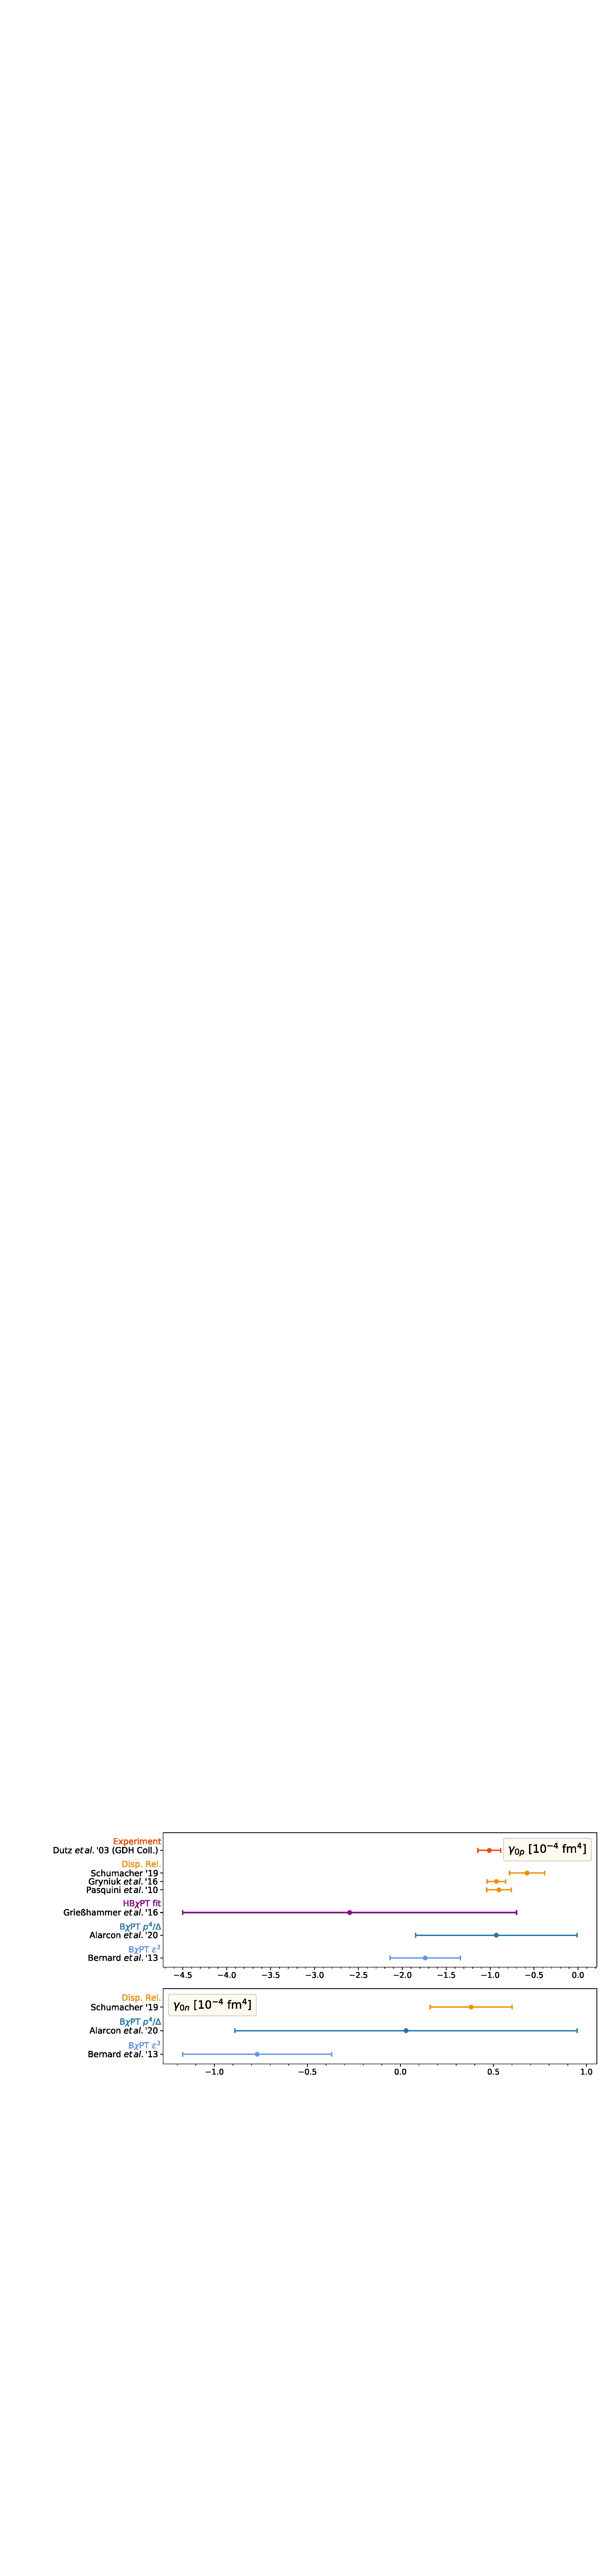
\includegraphics[width=\columnwidth]{Figures/Gamma0Pol.pdf}
\caption{Forward spin polarizability $\ga_0$ of the nucleon. \label{Gamma0Pol}}
\end{figure} 







Most recent HB$\chi$PT \cite{McGovern:2012ew,Griesshammer:2012we,Griesshammer:2015ahu} and B$\chi$PT \cite{Lensky:2008re,Lensky:2009uv,Lensky:2014efa, Lensky:2014dda,Lensky:2015awa,Lensky:2016nui,Alarcon:2020wjg, Alarcon:2020icz} calculations and fits of
CS observables employ the 
$\de$-expansion power counting. An exception is the work of Bernard et al.\ \cite{Bernard:2012hb}. As one can see from Figure~\ref{LTPolarizabilities}, B$\chi$PT predictions for $\delta_{LTp}$ within the $\delta$-expansion \cite{Lensky:2014dda,Alarcon:2020icz} or the $\epsilon$-expansion \cite{Bernard:2012hb} deviate substantially, since they include the $\Delta(1232)$ in different ways. In the $\epsilon$-expansion, the longitudinal-transverse polarizability receives a large contribution from diagrams where the photons couple directly to the $\Delta(1232)$ inside a loop. These diagrams are absent in the $\delta$-expansion at $\mathcal{O}(p
^4/\varDelta)$, thus, there the effect of the $\Delta(1232)$ is small and agrees with the MAID model \cite{MAID}. For the generalized longitudinal-transverse polarizability $\delta_{LTp}(Q^2)$ a similar $Q^2$ evolution is found in both power-counting schemes. Therefore, the discrepancy found for the polarizability  $\delta_{LTp}$ at the real-photon point continues as a constant shift for all $Q^2$ \cite{Alarcon:2020icz}. Another difference between the B$\chi$PT calculations
\cite{Lensky:2015awa,Alarcon:2020icz,Bernard:2012hb} is the implementation of the magnetic-dipole $N$-to-$\Delta$ transition and the coupling $g_M$ \cite{Krebs:2019ddp}.

The $\mathcal{O}(p^4/\Delta)$ B$\chi$PT prediction \cite{Lensky:2015awa} and the B$\chi$PT fit \cite{Lensky:2014efa} of the proton dipole polarizabilities, see Figures~\ref{alphaE1Pol} and \ref{betaM1Pol}, are in good agreement. A HB$\chi$PT fit, which also includes the lowest-order spin polarizabilities in Figures~\ref{ForwardSpinPolarizabilities} and \ref{Gamma0Pol}, agrees with the B$\chi$PT results \cite{Lensky:2015awa,Lensky:2014efa} except for $\ga_{M1E2}$. It is not possible to comment on the other HB$\chi$PT predictions for the dispersive, quadrupole and longitudinal polarizabilities \cite{Knoechlein97,Nevado:2007dd} since they have no error bars.\footnote{Note that the predictions for $M_1
^{(4)}$ and $\al_L$ were extracted from the VVCS amplitudes presented in Ref.~\cite{Nevado:2007dd}, but are not quoted in the original work.}
 


The most studied polarizabilities are the electric and magnetic dipole polarizabilities, for which the Particle Data Group publishes recommended values \cite{Zyla:2020}. They are needed as input for calculations of the proton-structure effects from two-photon exchange in the muonic-hydrogen Lamb shift. Of particular importance is $\beta_{M1p}$. It enters the $\ol T_1(0,Q^2)$ subtraction function \eref{subtractionfunction}, which has to be modeled \cite{Birse:2012eb} or predicted within $\chi$PT \cite{Alarcon:2020wjg,Lensky:2017bwi,Peset:2014jxa} because it cannot be measured in experiment or reconstructed from the unpolarized proton structure function $f_1$ in the dispersive approach. Recently,  $\beta_{M1p}$ has therefore been extracted from the linear polarization beam asymmetry,
\beq
\label{Eq:sigma_3}
\Si_3 = \frac{ \dd\sigma_{||} - \dd\sigma_{\perp} }{ 
\dd\sigma_{||} + \dd\sigma_{\perp} },
\eeq
 measured for the proton by the A2 Collaboration \cite{Sokhoyan:2016yrc} and LEGS \cite{Blanpied:2001ae}. Up to $\mathcal{O}(\nu^2$), the beam asymmetry $\Si_3$ provides access to 
$\beta_{M1}$ independent of $\alpha_{E1}$
\cite{Pascalutsa13}:
\begin{flalign}\label{Eq:krupina}
\ol \Si_3 = - 
\frac{4 M_N \omega_B^2 \cos\theta_B \sin^2\theta_B }{
 (1+\cos^2\theta_B)^2 }\, \alpha^{-1}\beta_{M1}.
\end{flalign}
Presently, the extraction of $\beta_{M1}$ from $\Sigma_3$  \cite{Sokhoyan:2016yrc} is not competitive with the standard dispersive analyses of unpolarized CS cross sections.
New high-precision measurements with significantly higher statistics should change this.

\begin{figure}[t]
\centering
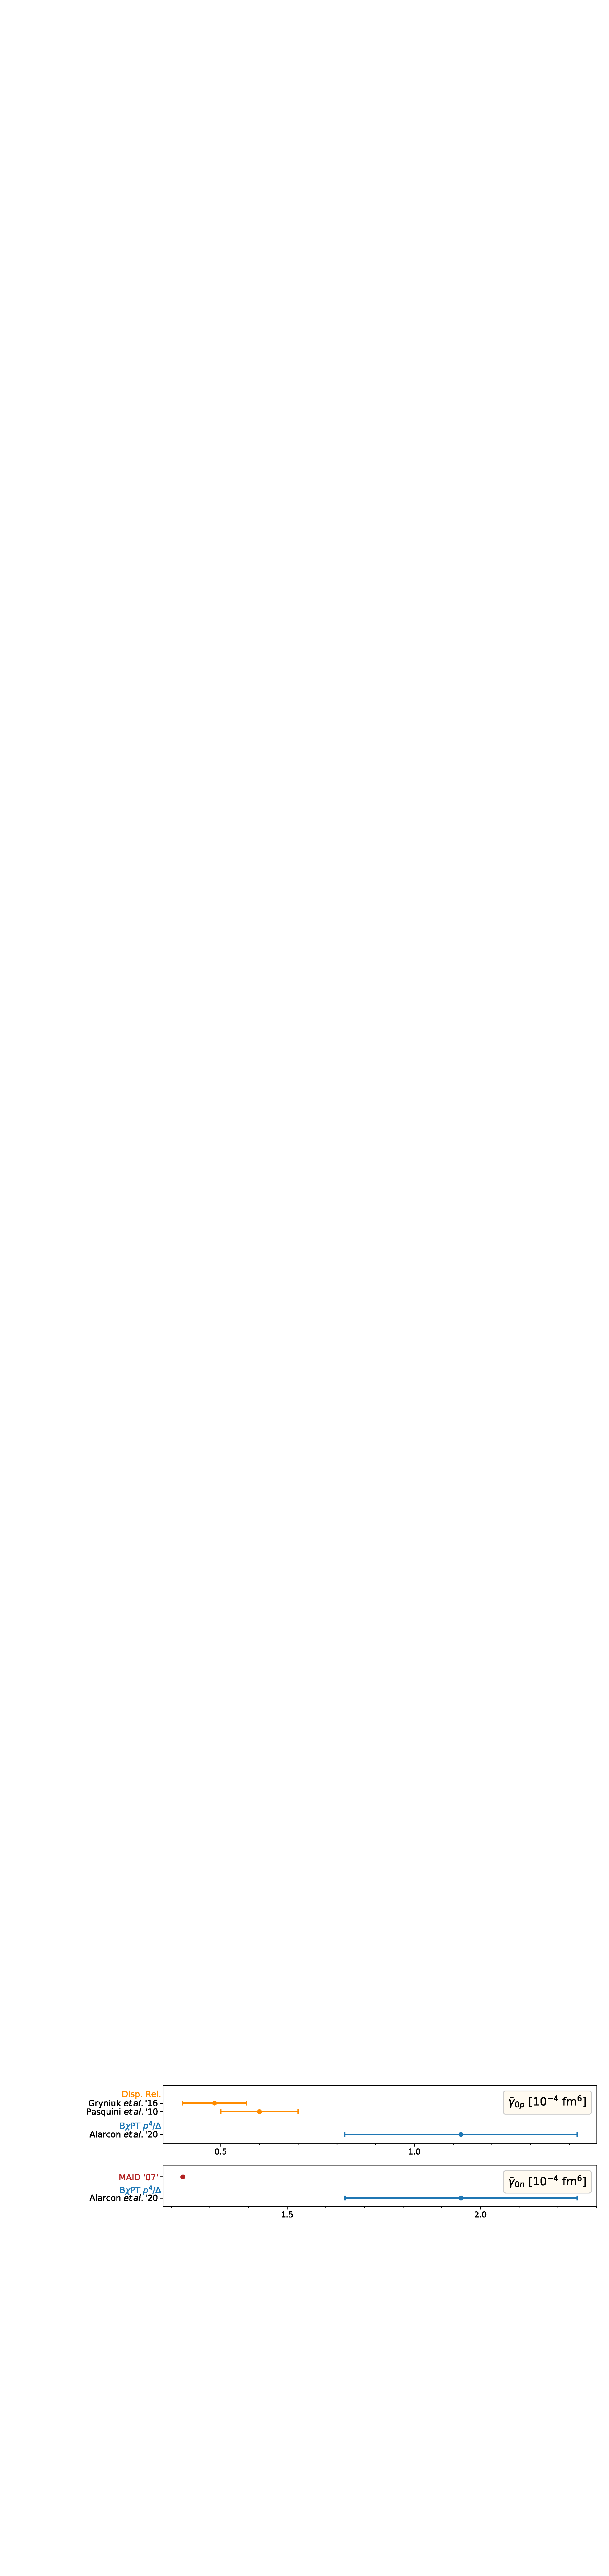
\includegraphics[width=\columnwidth]{Figures/BarGamma0Pol.pdf}
\caption{Fifth-order forward spin polarizability $\bar \ga_0$ of the nucleon. \label{BarGamma0Pol}}
\end{figure}

\begin{figure}[t]
\centering

\includegraphics[viewport=0 402 1115 700,clip,width=\columnwidth]{Figures/AllPolarizabilities05.pdf}
%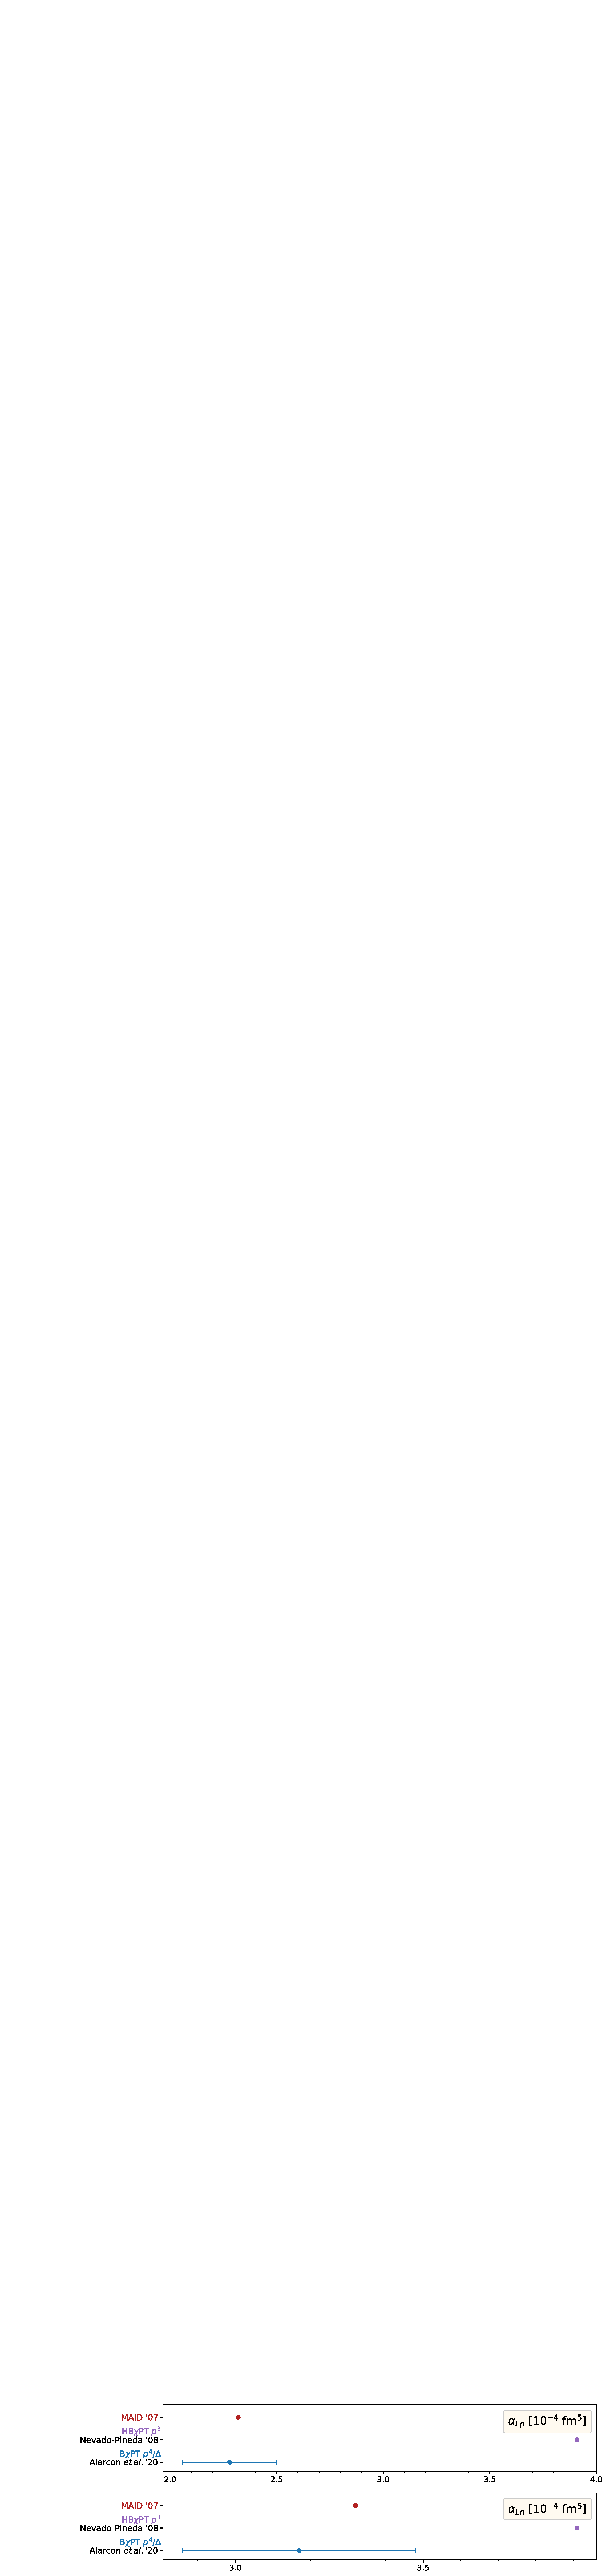
\includegraphics[width=\columnwidth]{Figures/LongitudinalPolarizability.pdf}
\caption{Longitudinal polarizability $\al_{L}$ of the nucleon. \label{LongitudinalPolarizabilities}}
\end{figure} 



Analyses of CS data with fixed-$t$ unsubtracted dispersion relations can be found in Refs.~\cite{Schumacher:2005an,Babusci:1998ww}, with an update in Ref.~\cite{Schumacher:2019ikn}. Fixed-$t$ subtracted dispersion relations are used in Ref.~\cite{Holstein:1999uu}, and are applied together with a bootstrap-based fitting technique in the recent Ref.~\cite{Pasquini:2019nnx}. Unfortunately, the dispersive and $\chi$PT fits tend to disagree for certain polarizabilities, e.g., for  $\al_{E1p}$ and $\beta_{M1p}$, cf.\ Figures~\ref{alphaE1Pol} and \ref{betaM1Pol}. Recently, an independent 
partial-wave analysis of proton RCS data below pion-production threshold has shown that the differences between dispersive approaches and B$\chi$PT extractions are due to inconsistent experimental data subsets and not a sign of ``model-dependence'' \cite{Krupina:2017pgr}. From this work, the result (Fit 0) of fitting the complete database with the dipole and lowest-order spin polarizabilities, cf.\ Figure
~\ref{ForwardSpinPolarizabilities}, as free parameters and the customary constraints from the data-driven evaluations of the Baldin and forward spin polarizability sum rules \cite{Gryniuk:2016gnm, Gryniuk:2015eza} is shown in the summary figures. In Ref.~\cite{Pasquini:2017ehj}, the dipole dynamical polarizabilities entering the multipole decomposition of the scattering amplitudes were for the first time extracted from proton RCS data below pion-production threshold. At lowest order, they are related to the static dipole and dispersive polarizabilities, see Figure~\ref{DispersivePol}. 

Both Ref.~\cite{Krupina:2017pgr} and Ref.~\cite{Pasquini:2017ehj} conclude that quantity and quality of the data has to increase for improved extractions of the nucleon polarizabilities. A trend is going towards the measurement of beam asymmetries, such as $\Sigma_3$, and double-polarization observables:
\begin{subequations}
\bea
\Sigma_{2x} &=& {  \dd\sigma^R_{+x}  -   \dd\sigma^L_{+x}   \over 
  \dd\sigma^R_{+x}  +  \dd\sigma^L_{+x}  },\\
\Sigma_{2z} &=& {  \dd\sigma^R_{+z}  -   \dd\sigma^L_{+z}   \over 
  \dd\sigma^R_{+z}  +  \dd\sigma^L_{+z}  },
\eea
\end{subequations}
where $\dd\sigma^{R(L)}_{+x}$ and $\dd\sigma^{R(L)}_{+z}$ are the differential cross sections for right (left) circularly polarized photons scattering from a nucleon target polarized either in the transverse $+\hat{x}$ direction or in the incident beam direction $+\hat{z}$. Here, the advantage is that systematic uncertainties, e.g., variations in photon flux or uncertainties in target thickness, are canceling out. Combining double-polarization observable and beam-asymmetry measurements, one is sensitive to the lowest-order spin polarizabilities, see Figure~\ref{ForwardSpinPolarizabilities}. For the extraction of the polarizabilities from the MAMI data for $\Sigma_{2x}$ \cite{Martel:2017pln,Martel:2014pba}, $\Sigma_{2z}$ \cite{Paudyal:2019mee} and $\Si_3$ \cite{Sokhoyan:2016yrc}, as well as the older LEGS data for $\Si_3$ \cite{Blanpied:2001ae}, one can use dispersive models \cite{Pasquini:2007hf,Holstein:1999uu,Drechsel:2002ar} or $\chi$PT fits \cite{Lensky:2009uv}.

Besides experimental efforts,
lattice QCD is making considerable progress. Most notably are the lattice QCD predictions for $\beta_{M1}$ with chiral extrapolation to physical pion mass \cite{Bignell:2018acn,Bignell:2020xkf}. As well as the plentiful results for $\al_{E1n}$ \cite{Lujan:2016ffj,Detmold:2010ts,Engelhardt:2007ub,Christensen:2004ca}. By now, even direct lattice evaluations of the unpolarized forward VVCS amplitude $T_1$ became possible and lead to predictions of the generalized Baldin sum rule and its fourth-order variant in the region of $Q
^2 \in \{ 2, 10\}$ GeV$^2$  \cite{Hannaford-Gunn:2020pvu,Chambers:2017dov}.

In Figures~\ref{Badlin4Pol}, \ref{Gamma0Pol}, \ref{BarGamma0Pol}, \ref{LongitudinalPolarizabilities} and \ref{LTPolarizabilities}, one can see updated results from the recent $\mathcal{O}(p^4/\Delta)$ B$\chi$PT prediction of unpolarized VVCS \cite{Alarcon:2020wjg}, related to $\al_L$ and $M_1^{(4)}$, and polarized VVCS \cite{Alarcon:2020icz}, related to $\delta_{LT}$, $\ga_0$ and $\bar \ga_0$. The latter could be compared to new results from the Jefferson Lab ``Spin Physics Program'' for the proton spin structure functions $g_1$ and $g_2$, see for instance the E08-027 experiment \cite{Zielinski:2017gwp} and the E97-110 experiment \cite{Sulkosky:2019zmn}. 

\begin{figure}[t]
\centering
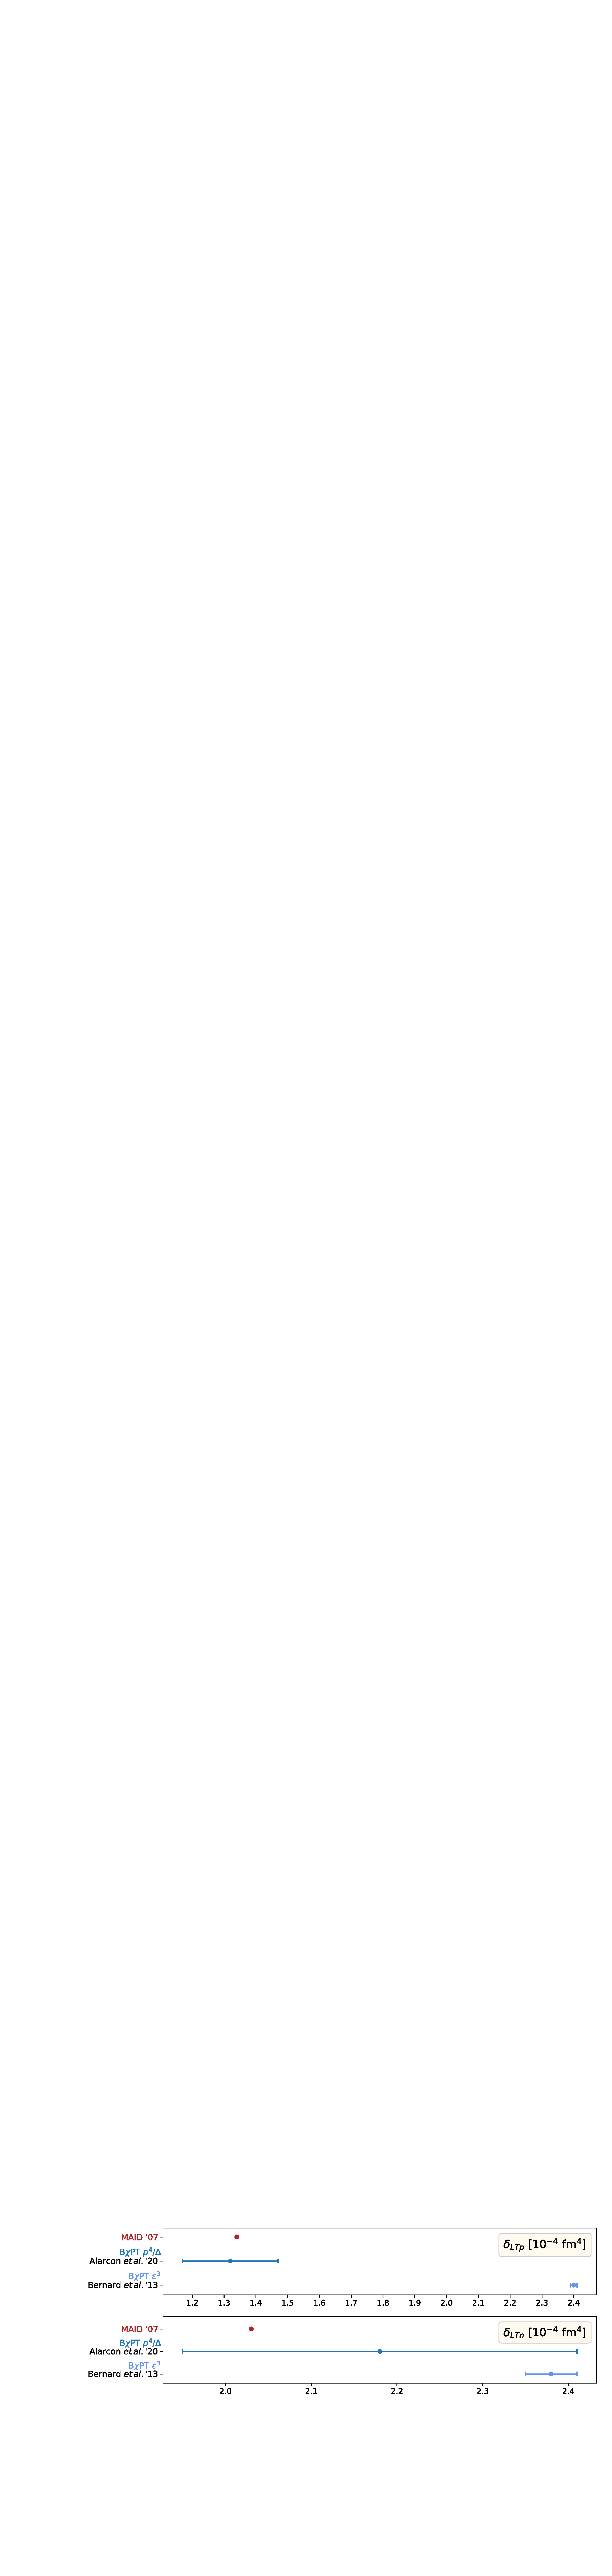
\includegraphics[width=\columnwidth]{Figures/LTPolarizabilities.pdf}
\caption{Longitudinal-transverse polarizability $\delta_{LT}$ of the nucleon. \label{LTPolarizabilities}}
\end{figure} 

\section{Summary and Conclusions} \label{hydrogen}

Chiral perturbation theory has predictive power for Compton scattering and the nucleon polarizabilities. Here, the chiral perturbation theory predictions have been compared to empirical determinations and lattice QCD predictions.  While most predictions agree with the experimental values, a few rather small discrepancies remain. To pin down the nucleon polarizabilities and resolve the present discrepancies, more high-precision data are needed. Here, a trend is going towards measurements of beam asymmetries or double-polarization observables with improved systematic uncertainties.
Chiral perturbation theory also provides a framework to fit low-energy Compton scattering data, and is used to design ``optimal experiments'' \cite{Melendez:2020ikd}.

Knowledge of the proton polarizabilities is  important as input for the proton-structure corrections to the muonic-hydrogen spectrum. These are not only relevant in the context of the proton-radius puzzle \cite{Pohl:2010zza,Antognini:1900ns}, but also for the planned measurements of the muonic-hydrogen ground-state hyperfine splitting \cite{Pohl:2016xsr,Bakalov:2015xya,Kanda:2018oay}.



\vspace{6pt} 

\funding{Financial support from the Swiss National Science Foundation is gratefully acknowledged.}

\acknowledgments{I would like to thank Jose~M.~Alarc{\'o}n, Vadim~Lensky, Vladimr~Pascalutsa and Marc~Vanderhaeghen for the fruitful collaboration on this topic, and Gilberto~Colangelo for many useful remarks on the manuscript. }


\abbreviations{The following abbreviations are used in this manuscript:\\

\noindent 
\begin{tabular}{@{}ll}
B$\chi$PT & Baryon chiral perturbation theory\\
$\chi$PT & Chiral perturbation theory\\
CS & Compton scattering\\
EFT & Effective-field theory\\
HB$\chi$PT & Heavy-baryon chiral perturbation theory\\
LEC & Low-energy constant\\
RCS & Real Compton scattering\\
VCS & Virtual Compton scattering\\
VVCS & Forward doubly-virtual Compton scattering\\
\end{tabular}}



\reftitle{References}
\bibliography{lowQ}


\end{document}

